% this file is called up by thesis.tex
% content in this file will be fed into the main document
\ifpdf
    \graphicspath{{figures/}{figures/comparisons}}
\else
    \graphicspath{{figures/}{figures/comparisons}}
\fi

%: ----------------------- name of chapter  -------------------------
\chapter{Reconstruction using only Sensor Fusion data}\label{chap:recon_sensors}
Initially, the author assumed the usage of the camera rotation and translation estimations from Android Sensor Fusion data only for 3D reconstruction purposes. However, the first attempts to perform reconstruction proved it to be not sufficient and additional rotation error matrix estimations were developed. Unfortunately when it comes to relying on hand-held smartphones, the collected sensor data are very noisy. This chapters explains the concept of how Sensor Fusion can be used in order to obtain camera rotation and translation estimation. Then important implementation aspects behind those estimations are introduced and finally the results of conducted tests of rotation and translation accuracy are presented.
\section{Concept}
The internal camera parameters need to be calculated before the reconstruction process commences.
Where accurate rotations and translations of cameras are known, no additional pose calculations are needed. As shown in \ref{sec:points_triangulation} knowledge of rotation and translation between calibrated cameras is sufficient to perform triangulation in 3D reconstruction. While retrieving rotation from Android Sensor Fusion is quite easy (Sections \ref{sec:rot_cal} and \ref{sec:rot_gen}), it is harder to calculate translation. Android provides access to linear acceleration data, but to get translation it has to be double integrated over time (\ref{eq:trans_from_accel}).
\subsection{Heuristic for translation estimation}
Using the currently available Android sensor data it is difficult to estimate the relative translation of the device. First it has to be done continously, even between taking images. Also  linear acceleration measurements, which can be accessed with $Sensor.TYPE\_LINEAR\_ACCELERATION$ constant, are very noisy\cite{indoorPosition}. Such noisy data with double integration over time results in quite big errors after some time. First integration is required to acquire current velocity change and second integration over velocity is required to calculate position change in particular moment. 
However, it can be improved using human-walking model description with the following heuristic constraints over the calculated velocity:
\begin{enumerate}
\item When new linear acceleration sensor data is ready, first apply low pass filtering in order to reduce some high frequency noise. Every new linear acceleration value used for calculation should be weighted average of previous and current acceleration reading.  
\item Change sensor data vector from local camera coordinates to global reference system (multiply with inverted rotation matrix). Normally Android returns linear acceleration readings along device axes, using device rotation information they can be changed to readings that are independent from device current orientation. 
\item Decide depending on current state, if deviceMovementState has changed:
\begin{enumerate}
\item If device was previously IDLE and incoming Acceleration value is bigger than $0.5\frac{m}{s^2}$ change device state to MOVING and reset current velocity to $0\frac{m}{s}$
\item If device was previously MOVING and incoming Acceleration value is smaller than $0.1\frac{m}{s^2}$ change device state to IDLE
\end{enumerate}
\item Only if device is currently moving:
\begin{enumerate}
\item Update device velocity by multiplying current acceleration reading by time elapsed from previous reading (\ref{eq:velo_accel}). 
\item Check current speed with walk constraint and eventually scale it down to maximum walking speed value (People walk with average speed of $1.5\frac{m}{s}$)
\item Update device position according to equation \ref{eq:trans_from_accel}.
\end{enumerate}
\end{enumerate}
A code snippet of the described translation estimation heuristics from provided Android application can be found in listing \ref{lst:positionHeuristic}. Maximum walking speed can be adjusted, but by default it should be set to around $1.5\frac{m}{s}$ \cite{website:walkingSpeed}. 
The most important factor of the accurate reconstruction is correlation between movements in X,Y and Z axes. Noise in sensors is equally distributed on each axis, so its estimated translation should keep these movements' correlations properly.

\begin{lstlisting}[caption={Snippet from Android source code position estimation heuristic},label={lst:positionHeuristic},numbers=left,escapeinside={@}{@},float]
    public void onSensorChanged(SensorEvent event) {
            ...
        } else if (event.sensor == mLinearAcceleration) { 
            ...   
            //Filtering out some noise
            newGlobalAcceleration = lowPass(newGlobalAcceleration, currentGlobalAcceleration);
            //Switch linear acceleration from phone local coordinates to global coordinates
            Matrix.multiplyMV(newGlobalAcceleration, 0, invertedRotationMatrix.clone(), 0, newGlobalAcceleration, 0);

            double distance = getLength(currentGlobalAcceleration);
            long currentTimeMillis = System.currentTimeMillis();
            //Decide state of the device. Distance is in m/s^2
            if (distance > 0.5 && deviceState == State.IDLE) {
                if (currentTimeMillis - movingEndTime > 300) {
                    deviceState = State.MOVING;
                    currentGlobalVelocity = {0,0,0};
                }
            } else if (distance < 0.1 && deviceState == State.MOVING) {
                if (currentTimeMillis - movingStartTime > 350) {
                    deviceState = State.IDLE;
                }
            }

            if (deviceState == State.MOVING) {
                //Update current device velocity
                currentGlobalVelocity += currentGlobalAcceleration * dT;
                
                double velocity = getLength(currentGlobalVelocity);
                //Check and adjust current velocity. People walk with average speed 1.5\frac{m}{s}
                if (velocity > WALKING_MAX_VELOCITY) {
                    currentGlobalVelocity /= velocity / WALKING_MAX_VELOCITY;
                }
                
                //Update device relative position, s = V0 * t + a * t^2/2;
                currentRelativePosition += currentGlobalVelocity * dT + currentGlobalAcceleration * dT * dT / 2;                 
            }
            ...
    }   
\end{lstlisting}

\section{Evaluation}
In order to verify the accuracy of camera rotation and translation calculation using Sensor Fusion data additional specific tests were conducted. Few pictures were taken in special test environment with known camera translation between images and thus allowing to evaluate the differences between:
\begin{enumerate}
\item rotation calculated using 8-point algorithm from known image points,
\item rotation calculated using 8-point algorithm where to known points few outliers were added to see how exactly this affects rotation estimation.
\item rotation calculated from automatically matched points using standard OpenCV methods
\item rotation calculated directly from Sensor Fusion data.
\end{enumerate}
\subsection{Test Environment}
Pictures were taken from 9 different positions on 2x3m area. Those images can be found on attached CD in "DataSets" folder. Their positions and corresponding names are visualised in Figure \ref{fig:setup_schematic}. Grey and brown rectangles on this schematic represent photographed object and blue stars are position, from which images were taken. 
\begin{figure}[h!]
    \centering
    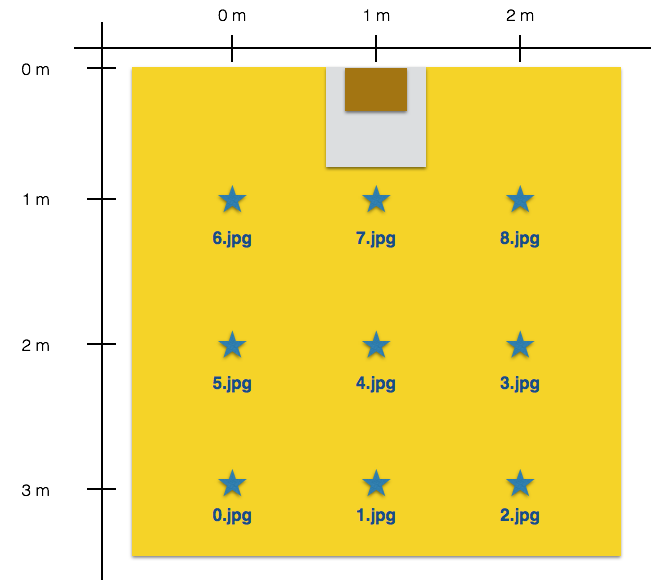
\includegraphics[width=0.8\textwidth]{setup_schematic}
    \caption[Schematic of test environment for capturing images along Sensor Fusion data]{Schematic of test environment for capturing images and Sensor Fusion data simultaneously. White and brown rectangles represent photographed object, blue stars with corresponding file name label positions from which test images were taken.}
    \label{fig:setup_schematic}
\end{figure}
In figure \ref{fig:setup_env_rot_test} it is shown how this setup environment looked in real life. Red circles indicate positions of visible markers, from which pictures were taken. 
\begin{figure}[h!]
    \centering
    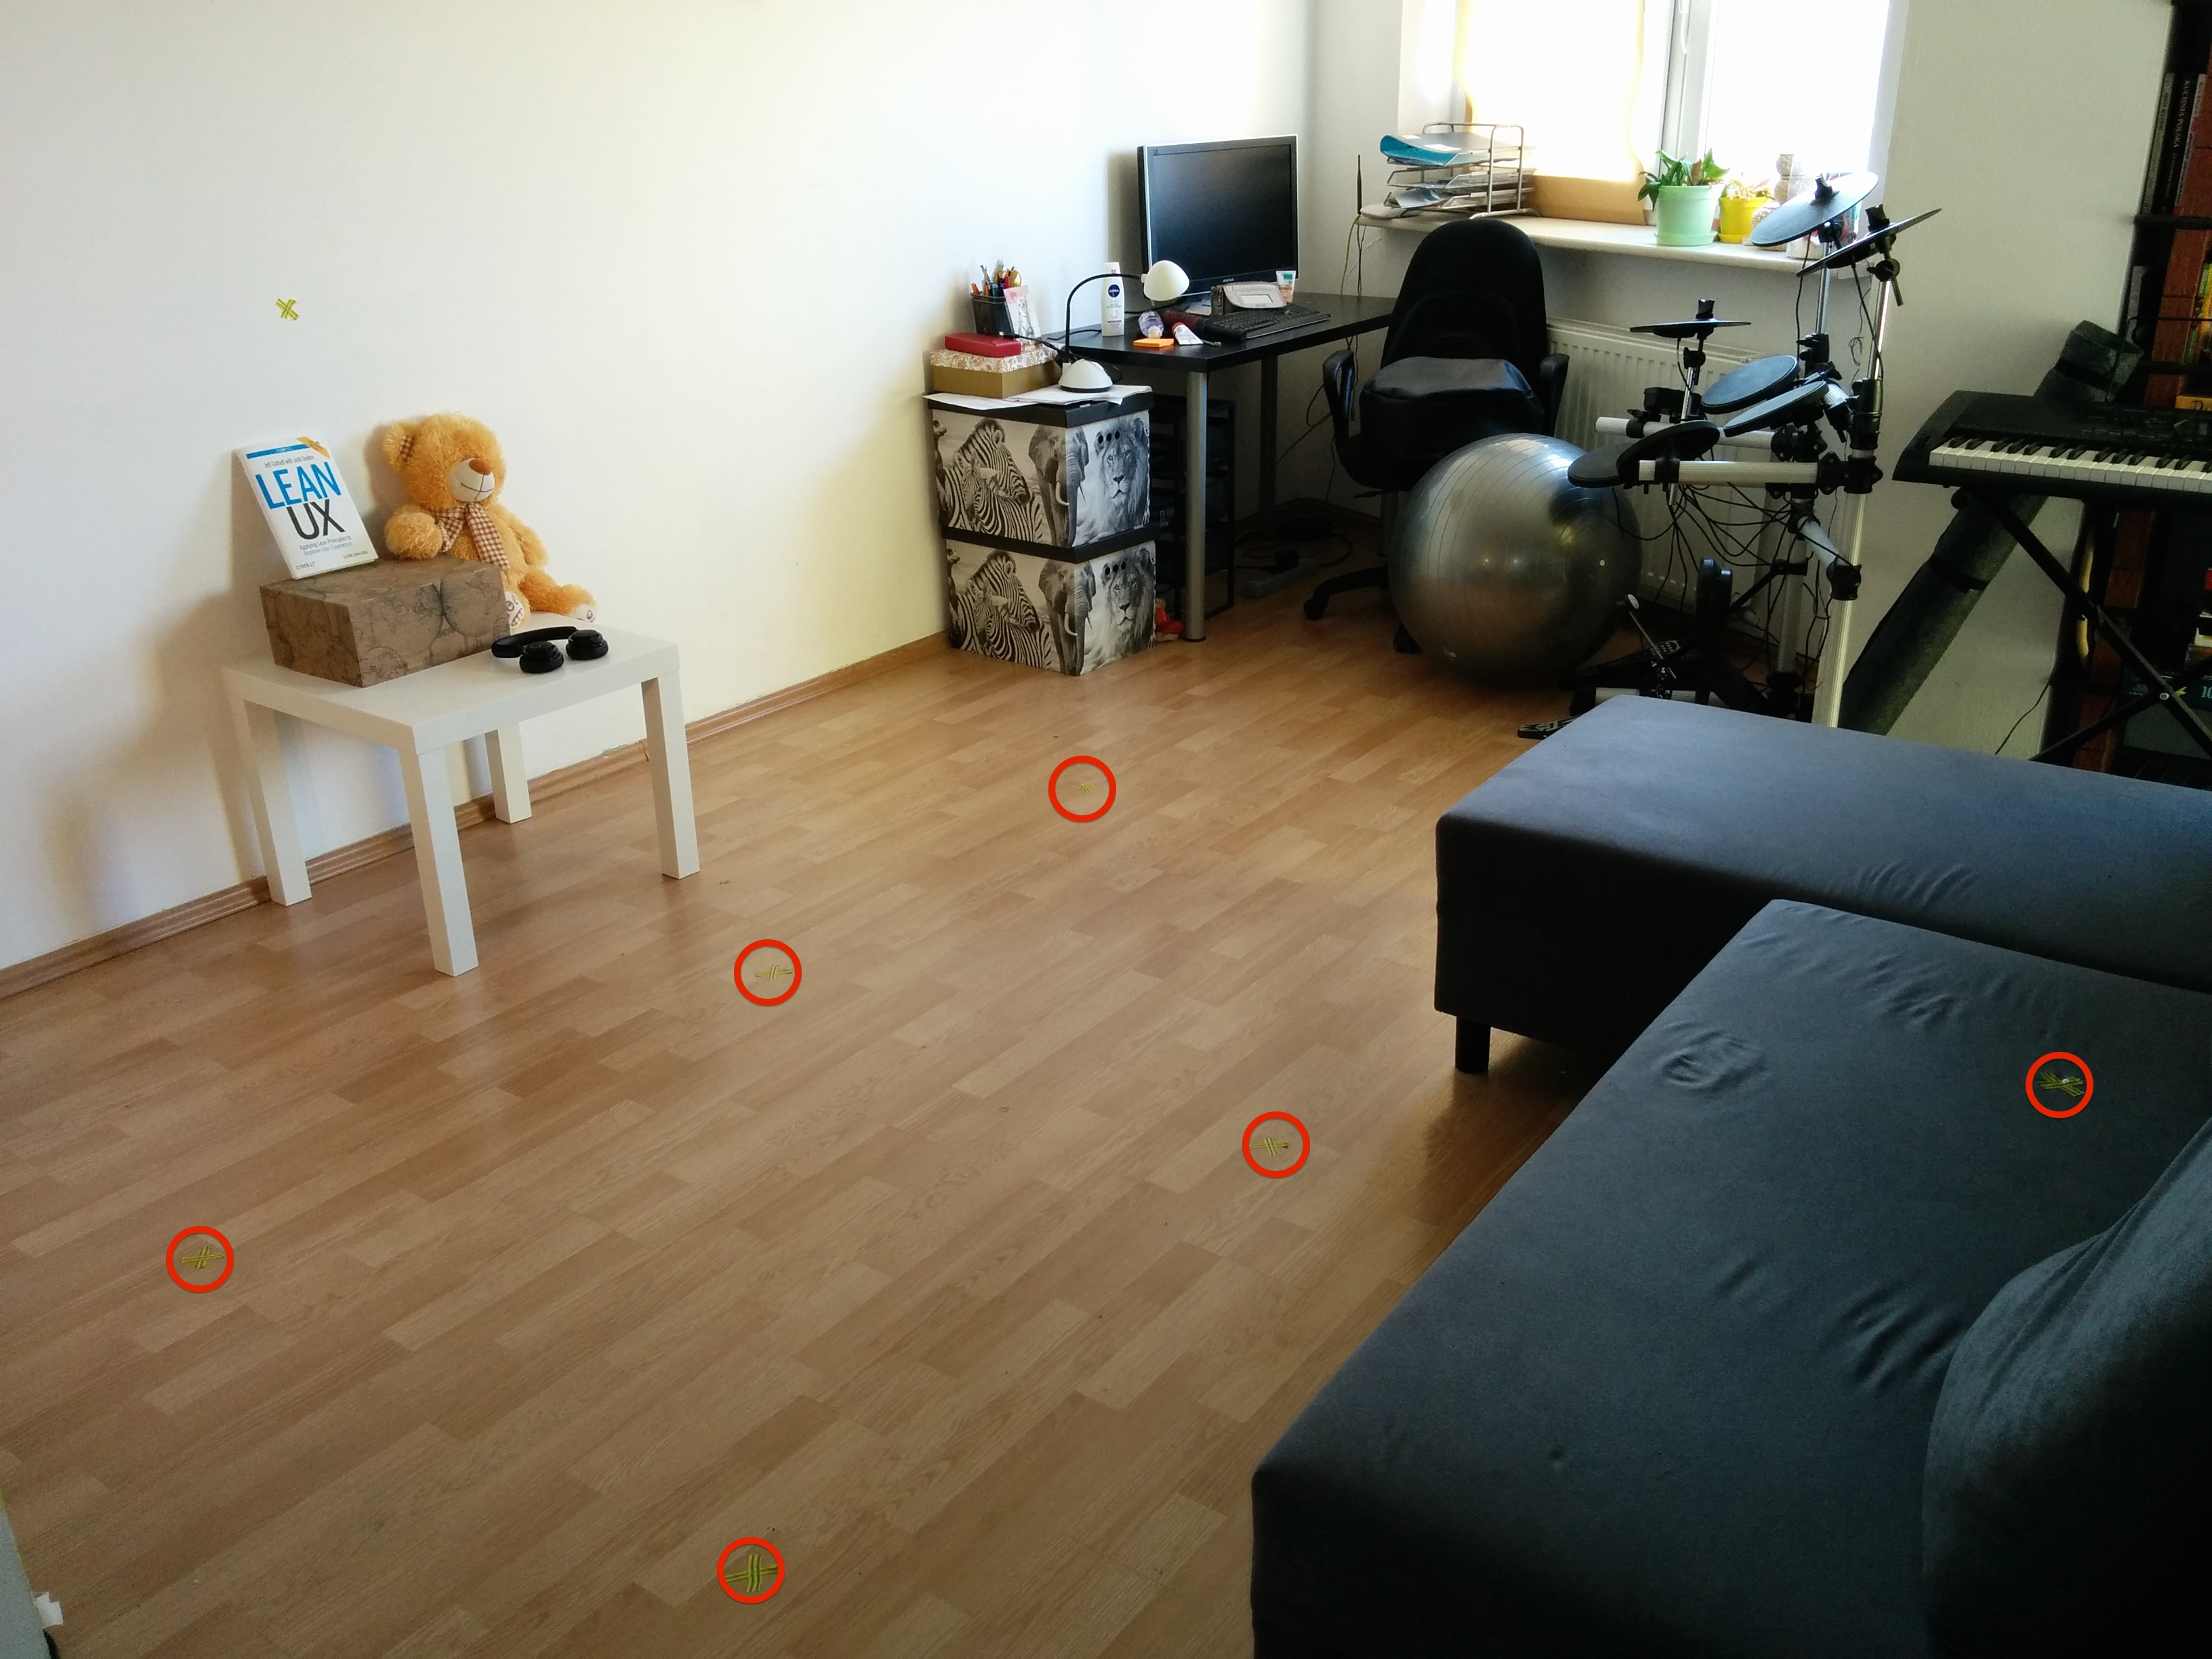
\includegraphics[width=0.8\textwidth]{setup_env_rot_test}
    \caption[Image of testing environment for capturing images along Sensor Fusion data]{Image of testing environment for capturing images along Sensor Fusion data. Red circles indicates positions of visible markers.}
    \label{fig:setup_env_rot_test}
\end{figure}
Marker used to note the capture positions can be seen in Figure \ref{fig:marker_env}.
\begin{figure}[h!]
    \centering
    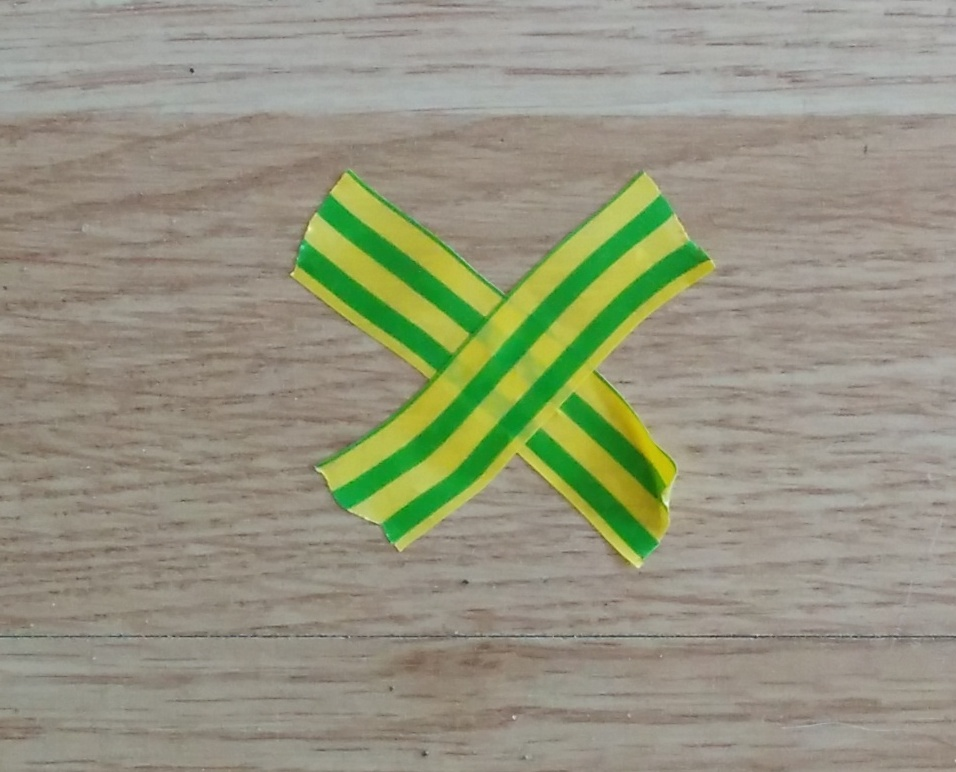
\includegraphics[width=0.4\textwidth]{marker_env}
    \caption{Image of marker used to indicate position for test capturing.}
    \label{fig:marker_env}
\end{figure}

\subsection{Rotation calculation tests}
After the pictures were taken many tests were made in order to verify, what differences one can expect in terms of rotation angles estimation. As mentioned four cases were researched:
\begin{enumerate} \label{enum:rotation_calcs_types}
\item Selecting proper corresponding points by user from image
\item Selecting proper corresponding points and adding few outliers by user
\item Automatic correspondence matching with SIFT descriptors and BruteForce matching from OpenCV
\item Rotation angles calculation directly from Sensor Fusion data
\end{enumerate}
In 4th case it was not necessary to calculate fundamental matrix and later decompose it to rotation angles. In others first fundamental matrix was calculated using standard 8-point algorithm implementation. In combination with internal camera matrix it allowed to calculate essential matrix. \textbf{E} was later was decomposed in the already described way to acquire proper rotation matrix. In figures \ref{fig:01_matching} - \ref{fig:01_matching_outliers} and \ref{fig:02_matching} - \ref{fig:02_matching_outliers} it can be seen, which points were selected by the author for two example image pairs to perform camera rotation estimation tests. In both cases red line means proper correspondence and yellow means improper match. In figures \ref{fig:f_01_auto_sift} and \ref{fig:f_02_auto_sift} reader can see, what types of results usually automatic matching produces. These results are quite good, but unfortunately have some outliers. 

\begin{figure}[h!]
    \centering
    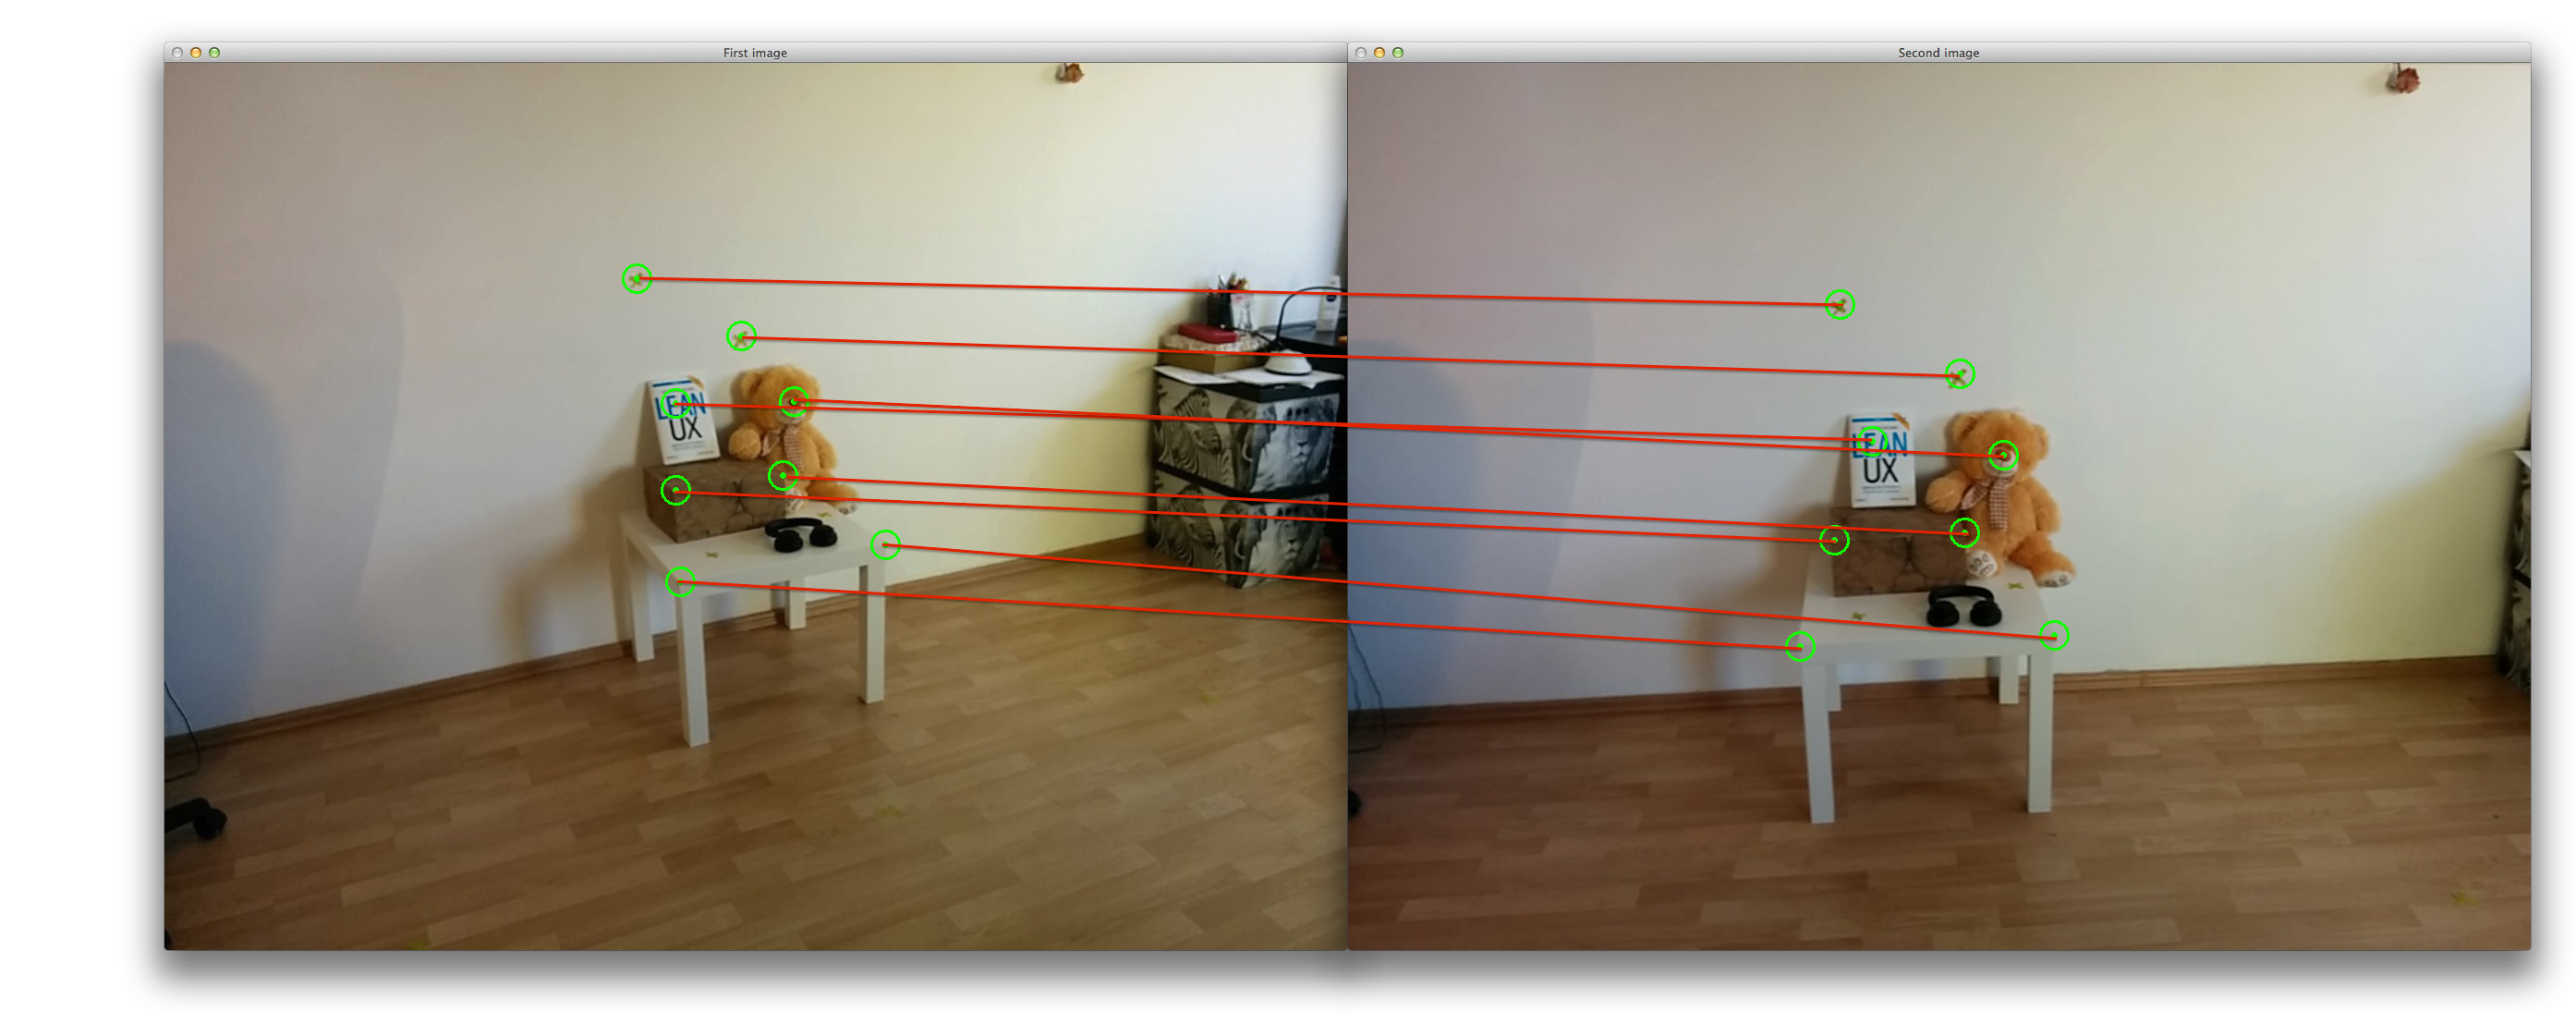
\includegraphics[width=0.8\textwidth]{01_matching}
    \caption{Points matches selected by the author (Images 0.jpg and 1.jpg).}
    \label{fig:01_matching}
\end{figure}
\begin{figure}[h!]
    \centering
    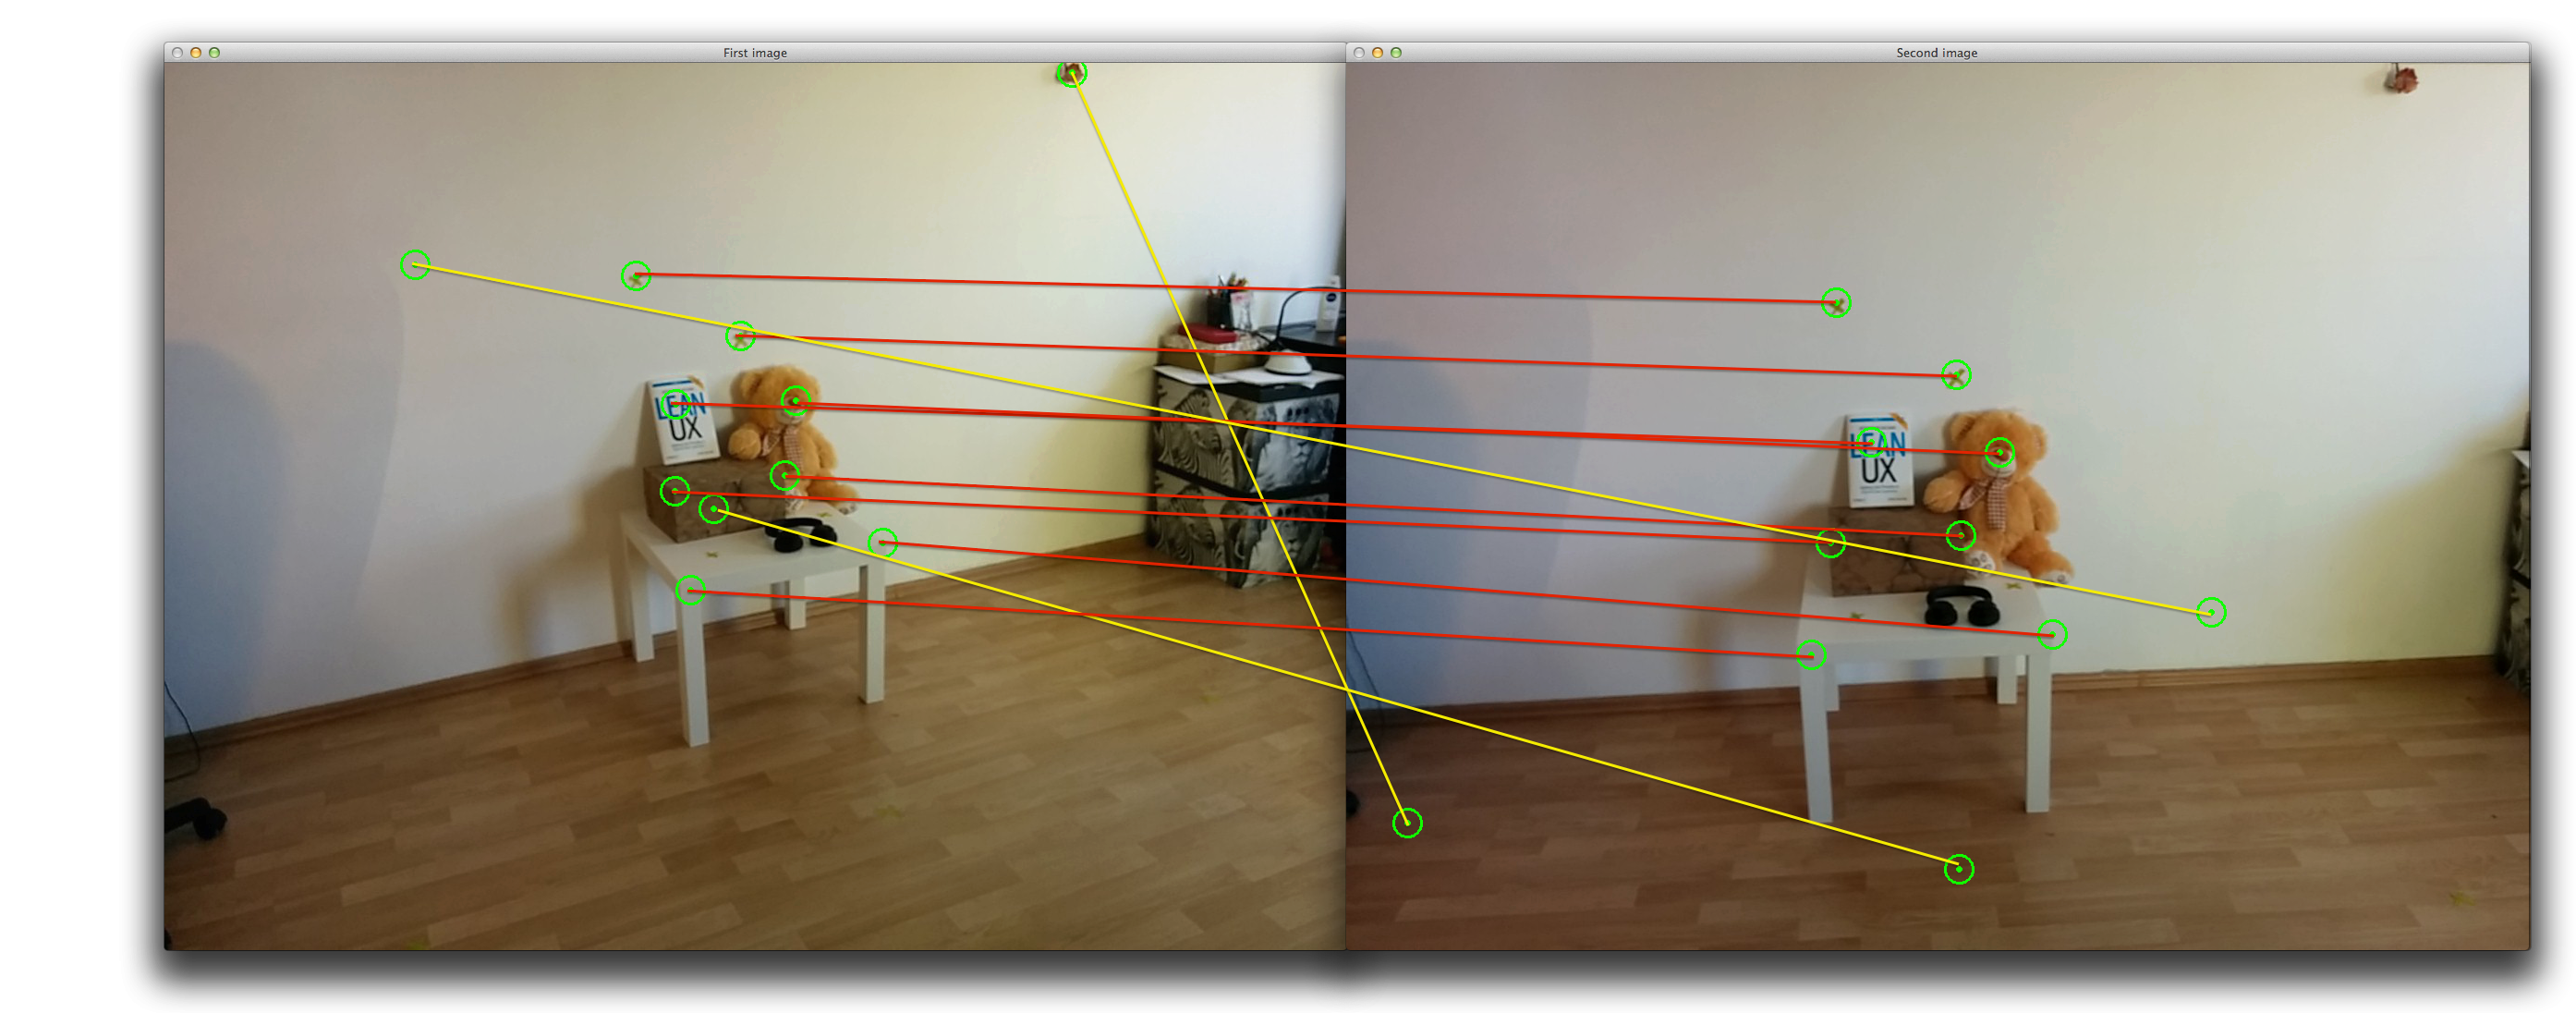
\includegraphics[width=0.8\textwidth]{01_matching_outliers}
    \caption{Points matches selected by the author with additional outliers (Images 0.jpg and 1.jpg).}
    \label{fig:01_matching_outliers}
\end{figure}
\begin{figure}[h!]
    \centering
    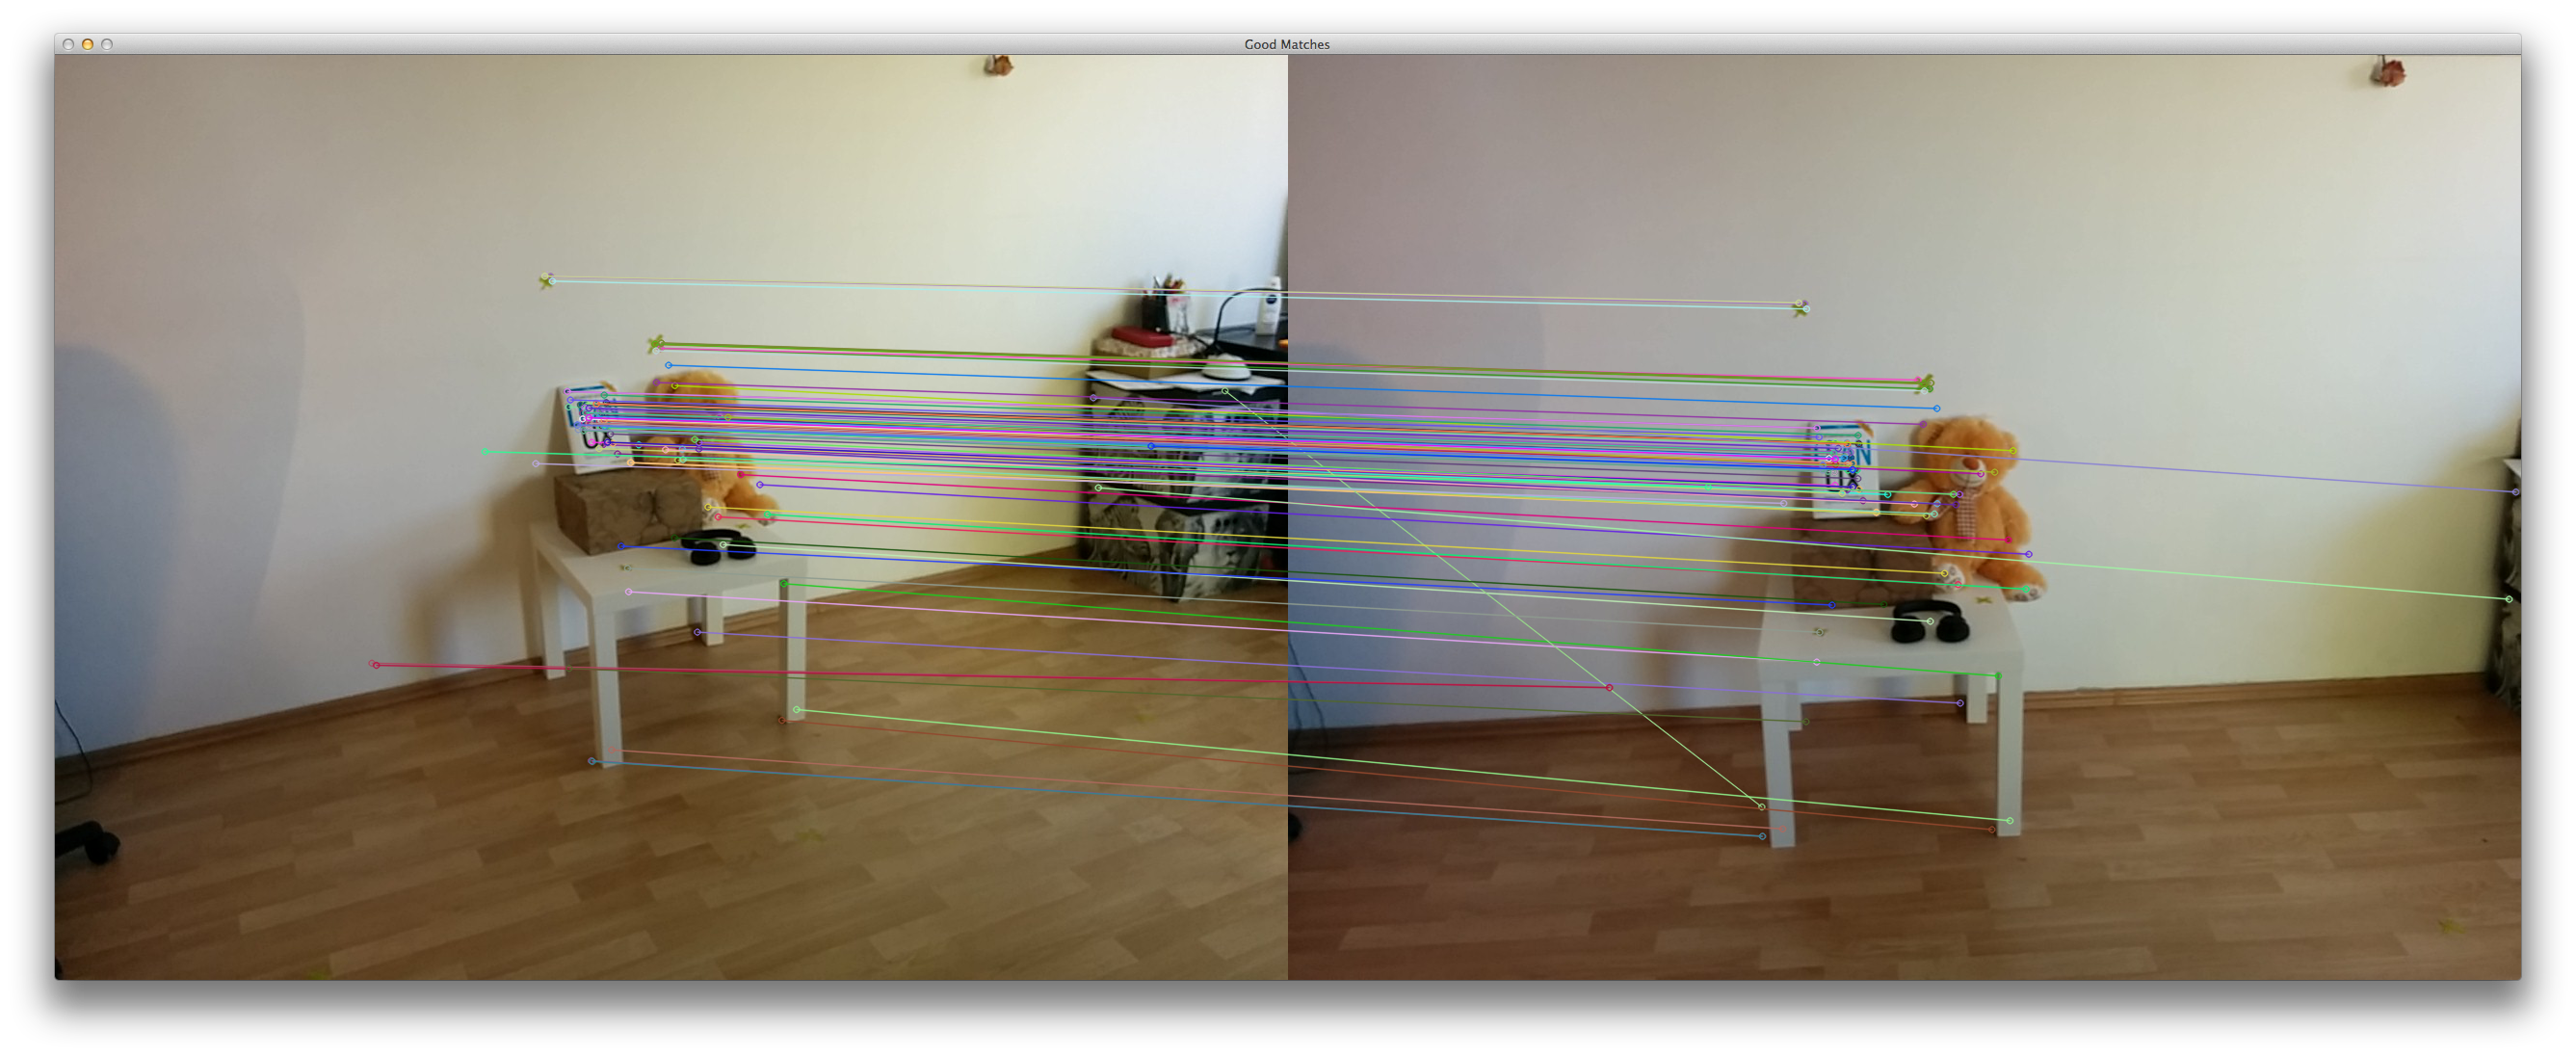
\includegraphics[width=0.8\textwidth]{f_01_auto_sift}
    \caption{Automatically matched points with usage of SIFT descriptors and BruteForce matcher (Images 0.jpg and 1.jpg).}
    \label{fig:f_01_auto_sift}
\end{figure}

\begin{figure}[h!]
    \centering
    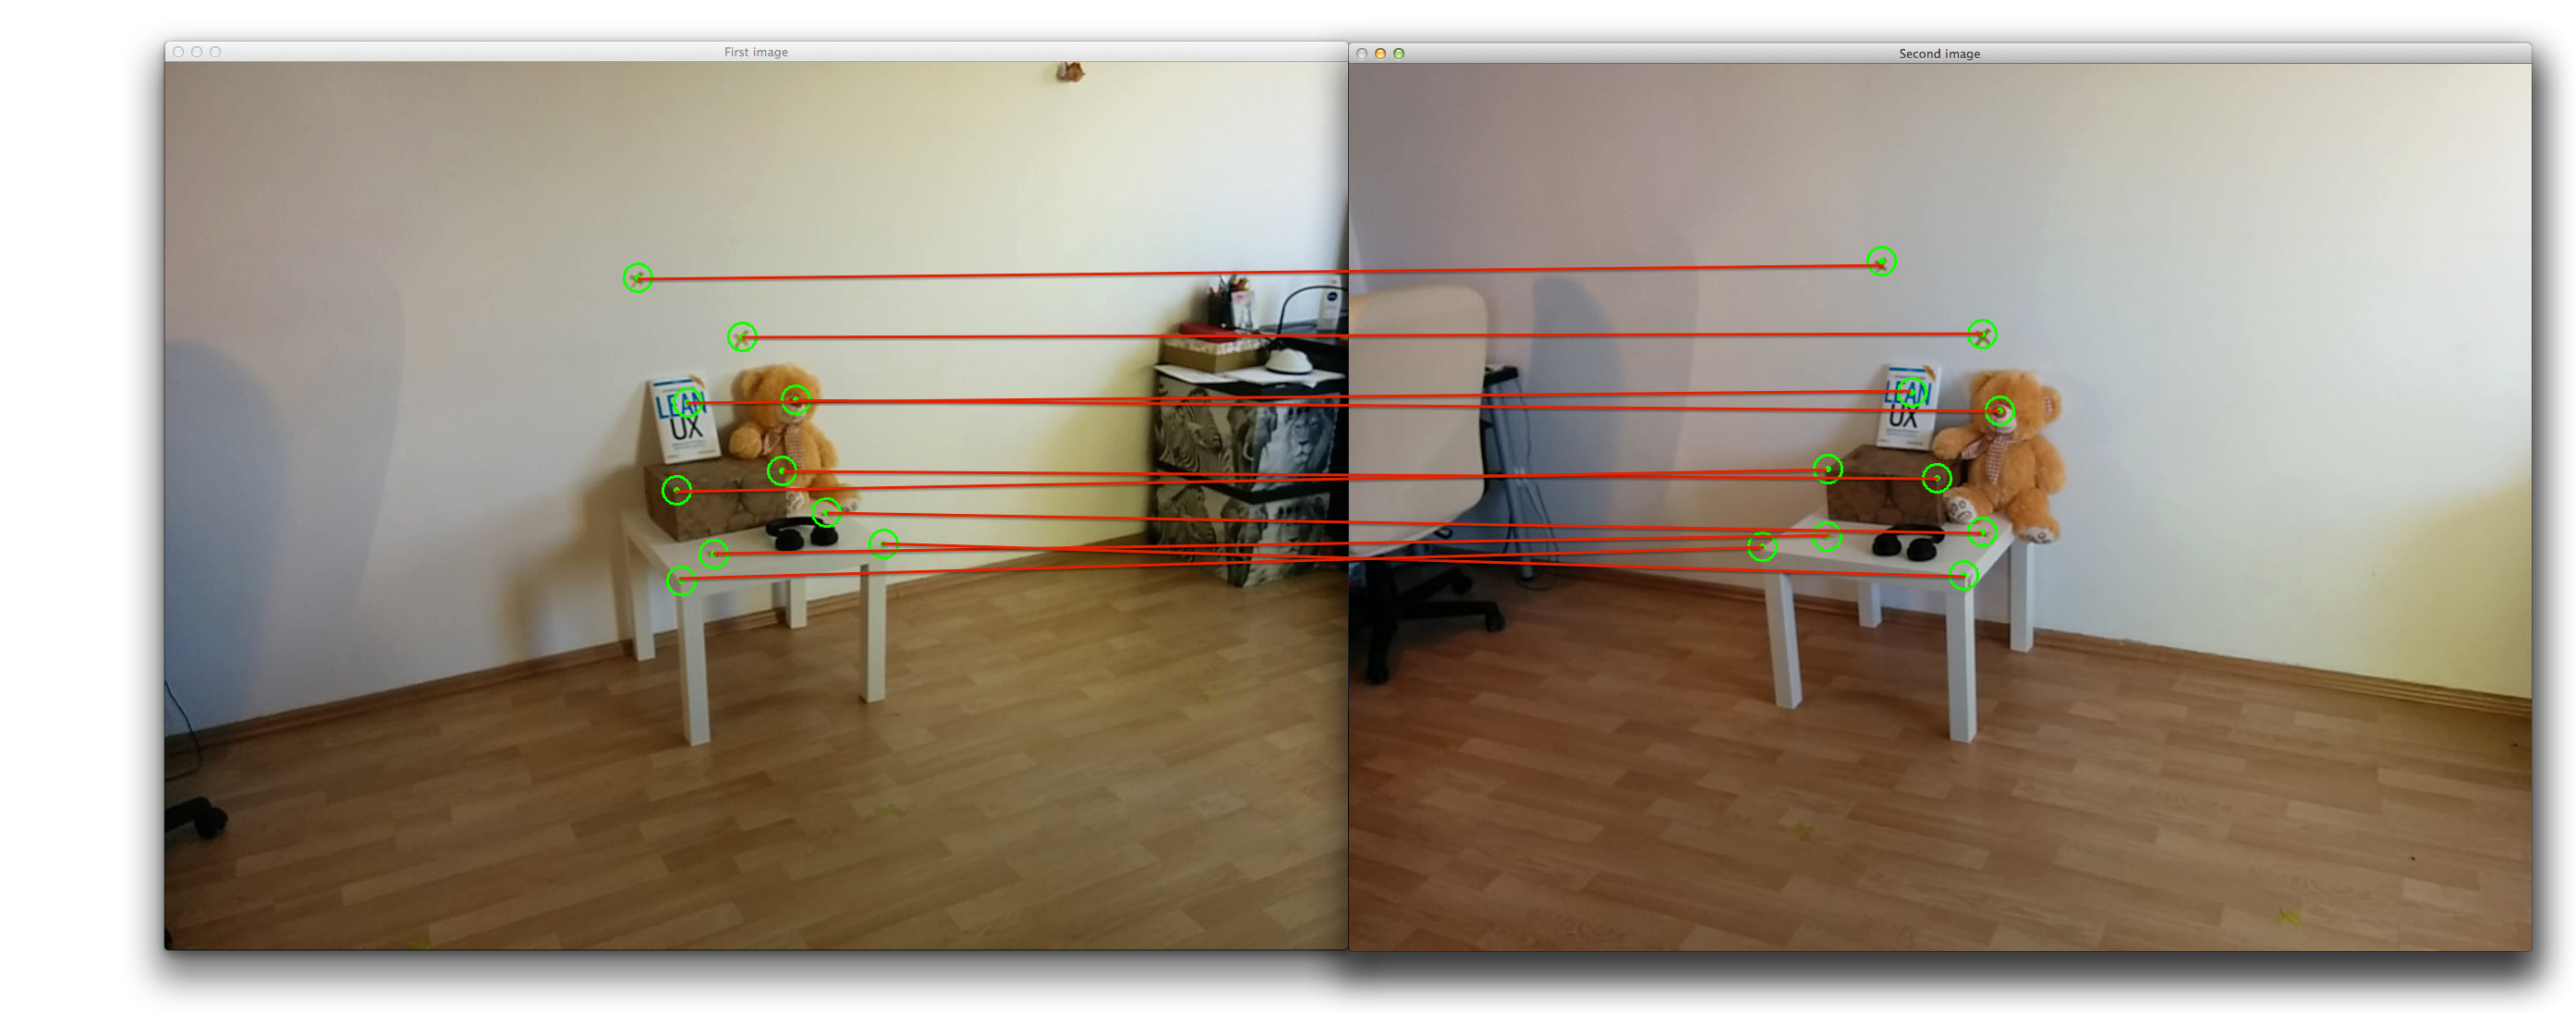
\includegraphics[width=0.8\textwidth]{02_matching}
    \caption{Points matches selected by the author (Images 0.jpg and 2.jpg).}
    \label{fig:02_matching}
\end{figure}
\begin{figure}[h!]
    \centering
    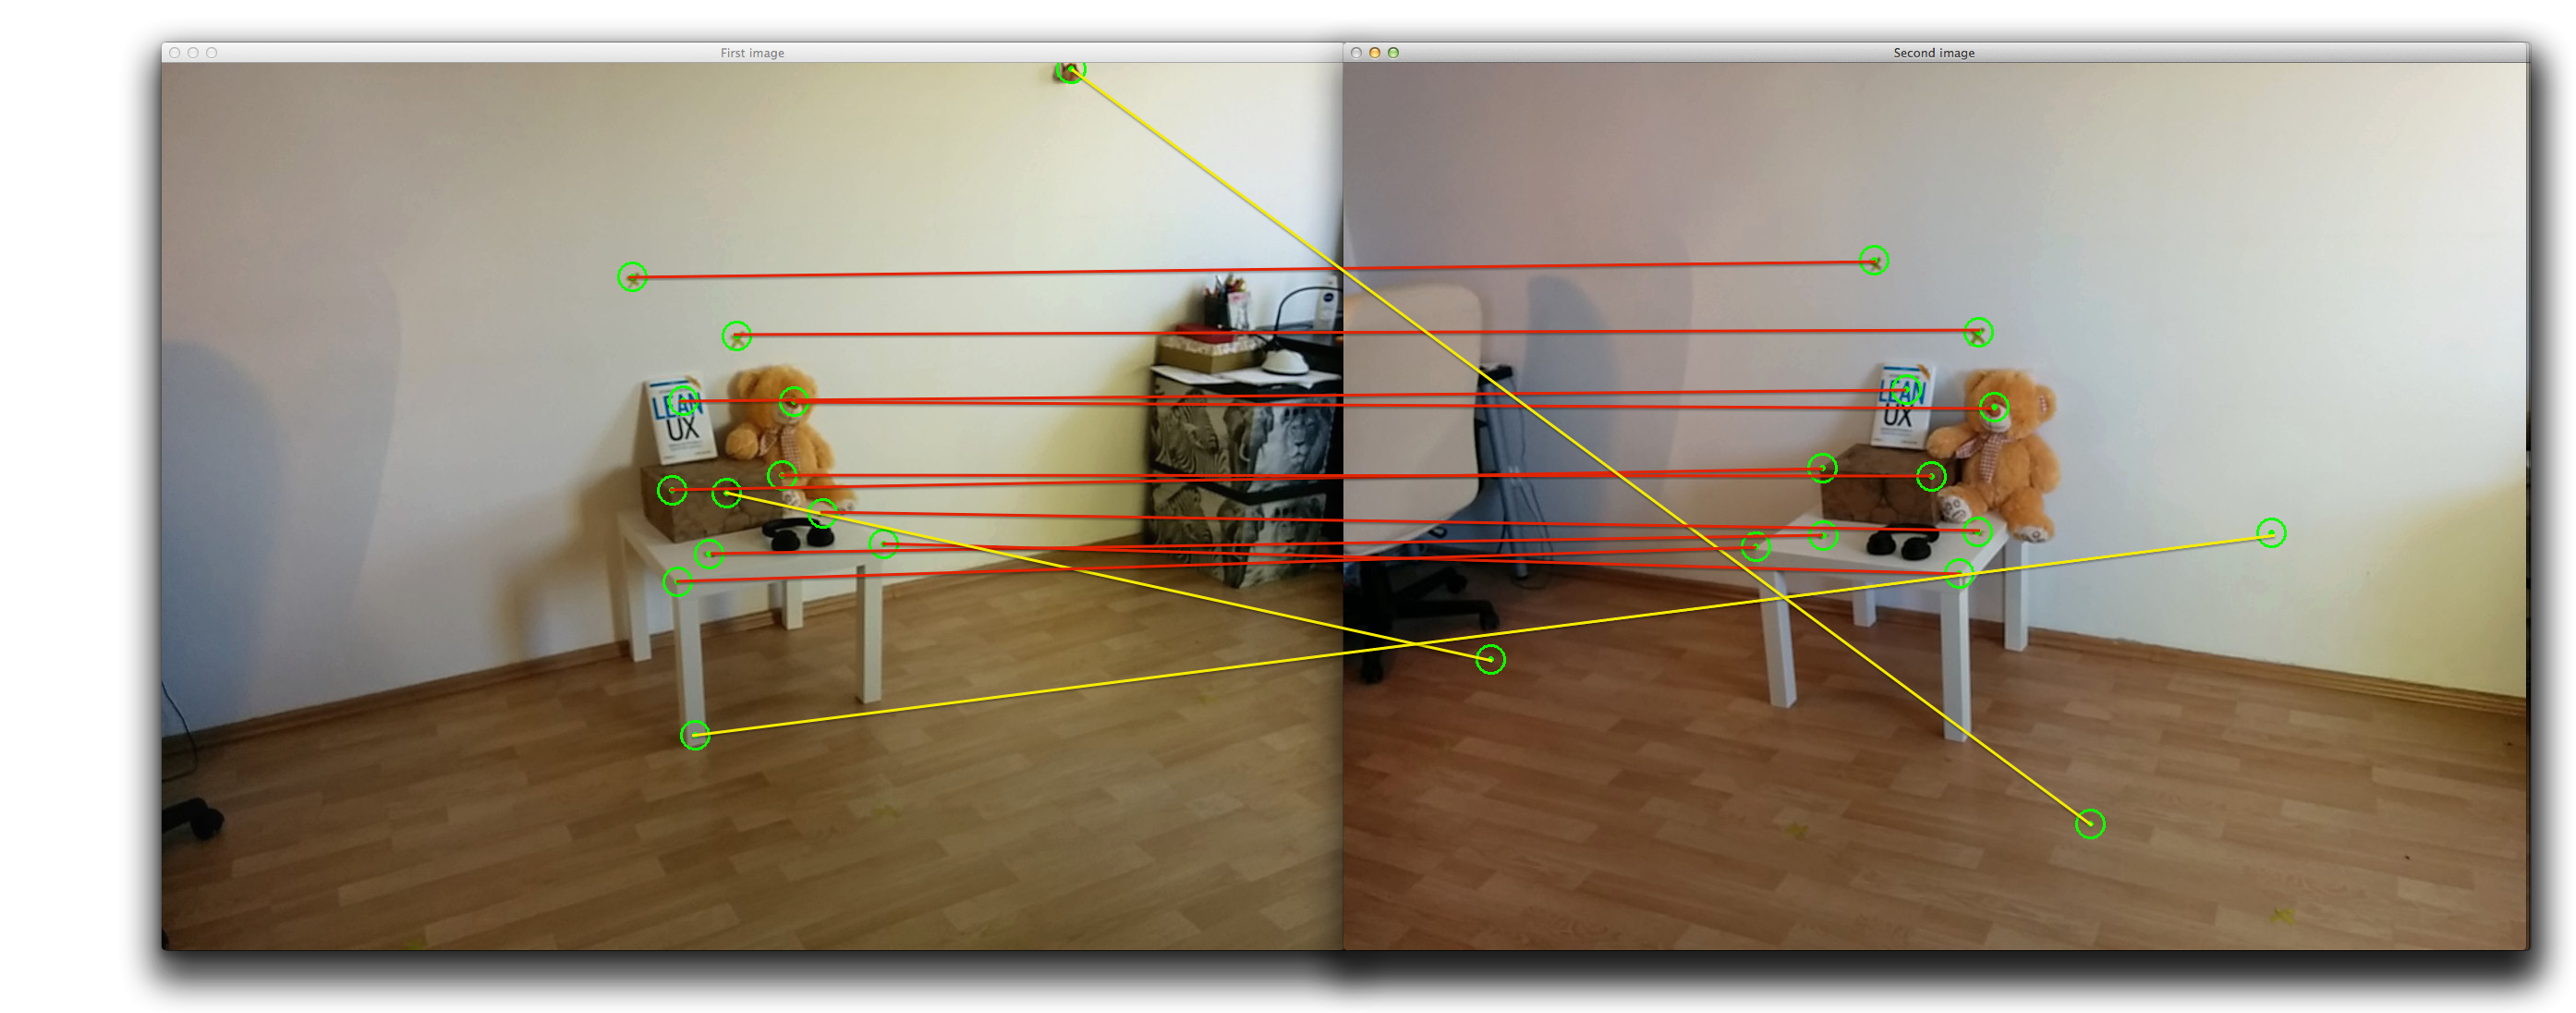
\includegraphics[width=0.8\textwidth]{02_matching_outliers}
    \caption{Points matches selected by the author with additional outliers (Images 0.jpg and 2.jpg).}
    \label{fig:02_matching_outliers}
\end{figure}

\begin{figure}[h!]
    \centering
    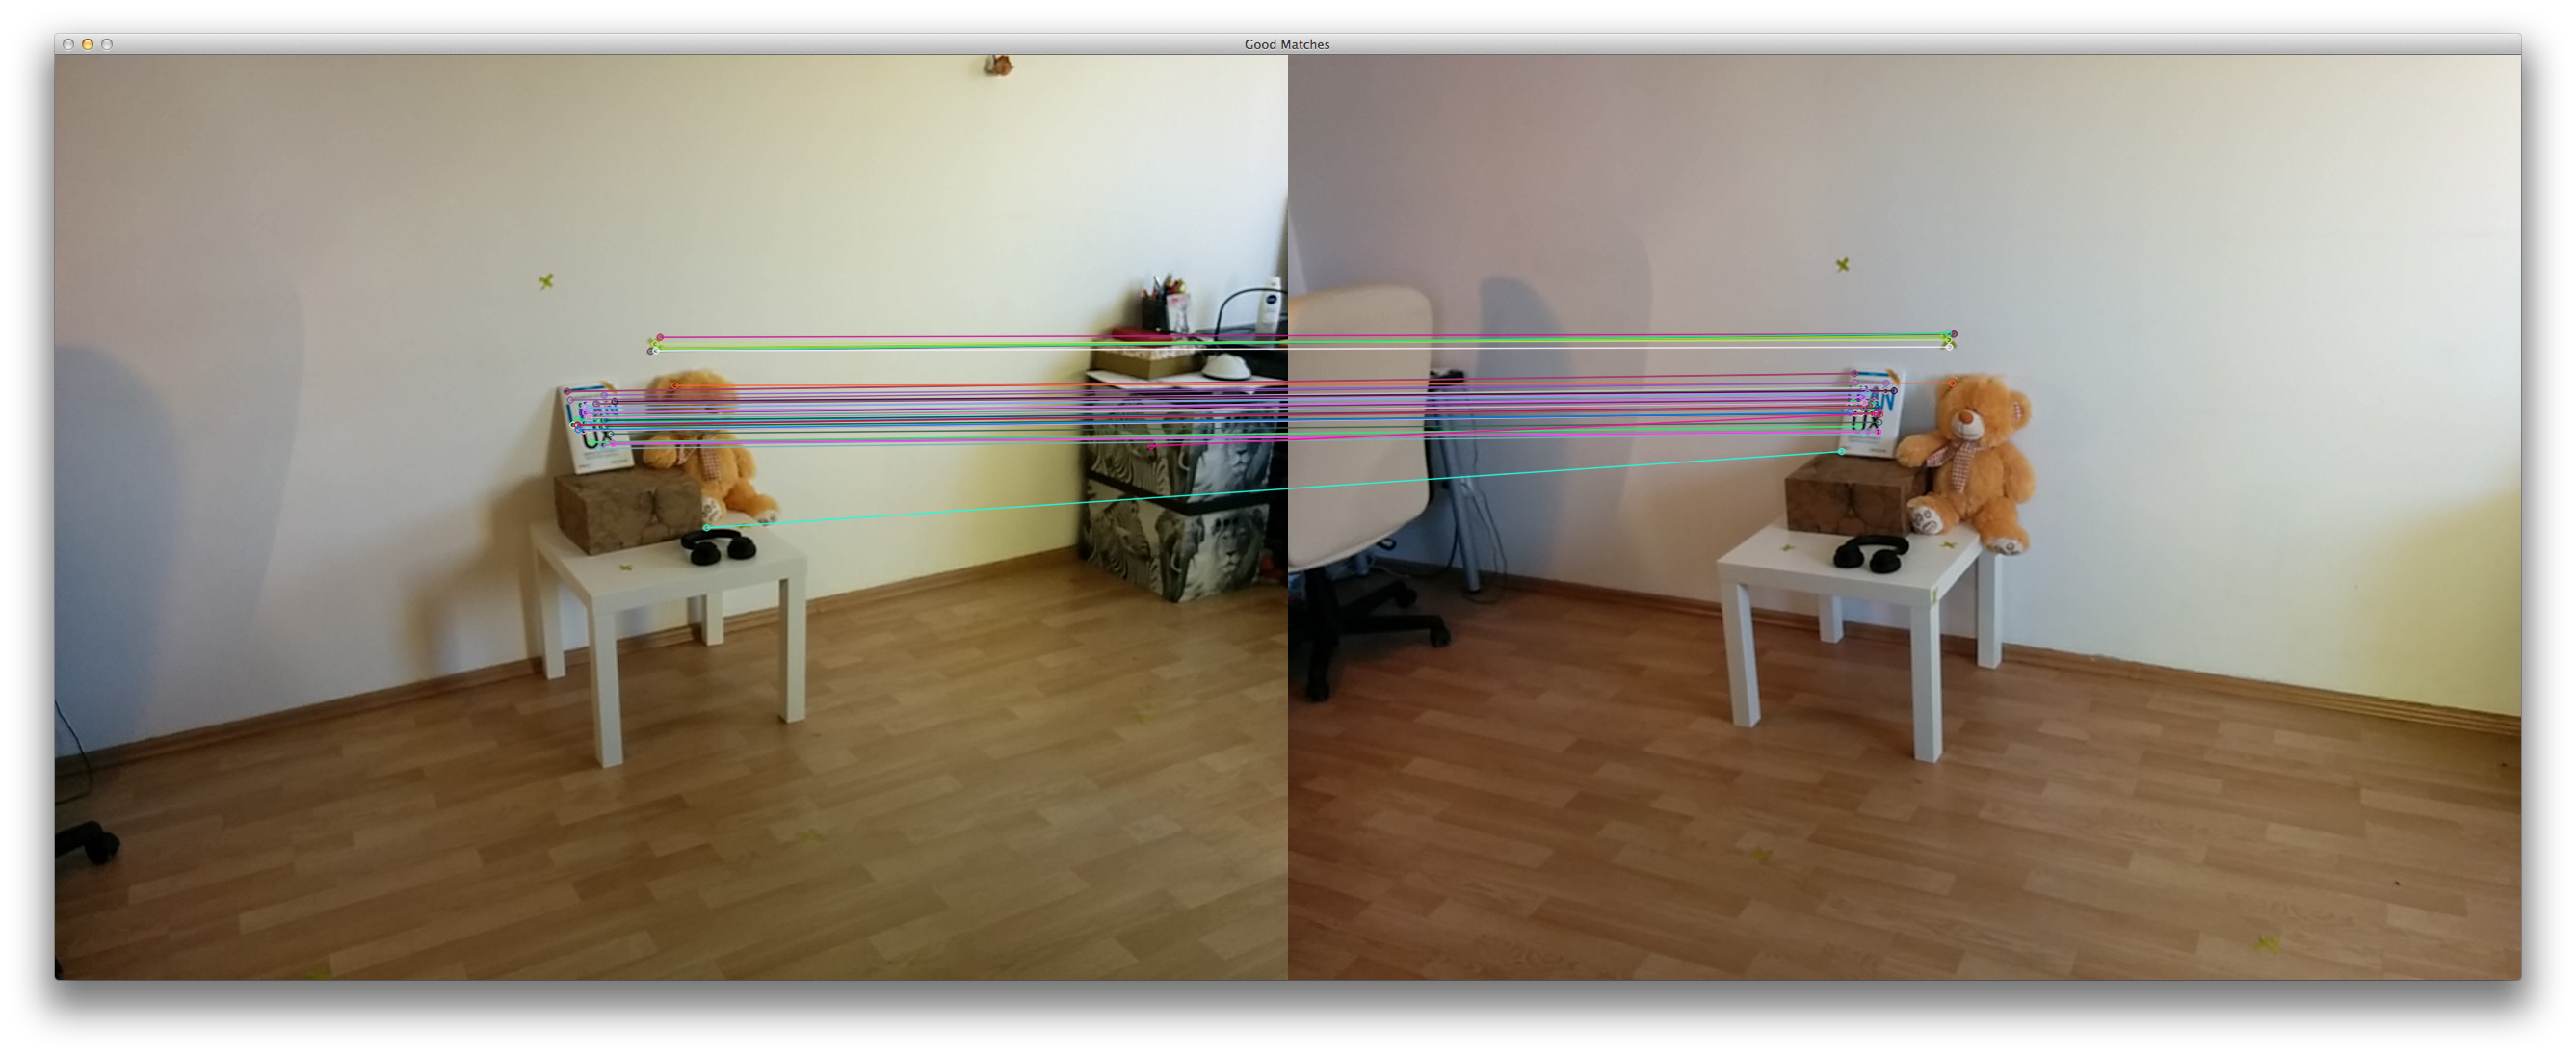
\includegraphics[width=0.8\textwidth]{f_02_auto_sift}
    \caption{Automatically matched points with usage of SIFT descriptors and BruteForce matcher (Images 0.jpg and 1.jpg).}
    \label{fig:f_02_auto_sift}
\end{figure}

For all mentioned in \ref{enum:rotation_calcs_types} situations corresponding F and E matrices were found and then they were decomposed to rotation matrices and finally transformed to Euler angles. In the following figures \ref{fig:rot_tests_01} and \ref{fig:rot_tests_02} these calculations were gathered. \\
In first row "known points" euler angles for proper user matching can be found. They also become the reference value for accuracy comparison for other cases. \\
What's important to notice that existence of only 3 outliers significantly influences the camera rotation estimation. Using data from sensors also doesn't give close enough approximation of angles, that would allow for building reconstruction algorithms relaying solely on them. \\
But of course to reconstruction camera translation information is needed. Next section will present effects of Sensor Fusion based approach to translation calculation.
\begin{figure}[h!]
    \centering
    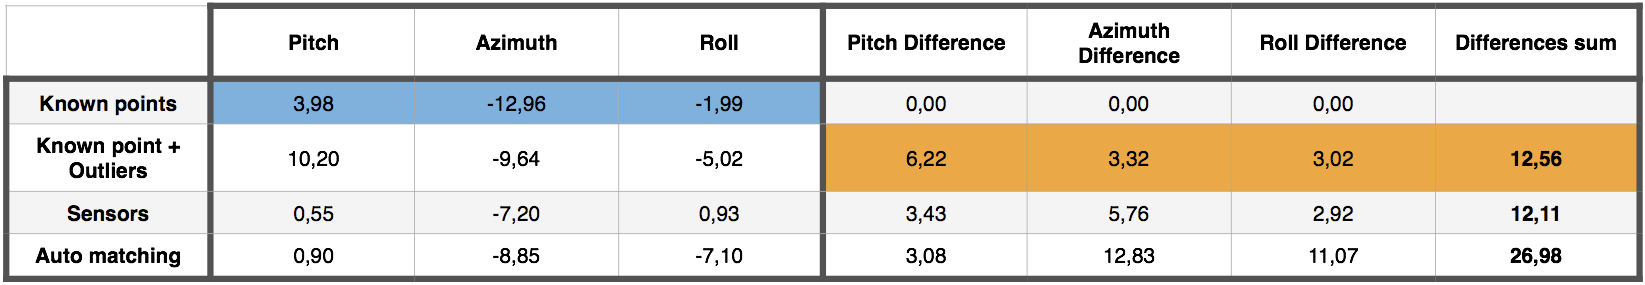
\includegraphics[width=0.95\textwidth]{rot_tests_01}
    \caption[Rotation tests comparison in Sensor only based approach - 1st example]{Rotation tests comparison in Sensor only based approach for 0.jpg and 1.jpg images. In first raw reference angles were calculated for proper point matching. Next raw shows how outliers influence those measurements. 3rd shows calculation using Sensor Fusion approach and 4th one measurements from automatic OpenCV supported matching. All angle differences are referenced to 1st row.}
    \label{fig:rot_tests_01}
\end{figure}
\begin{figure}[h!]
    \centering
    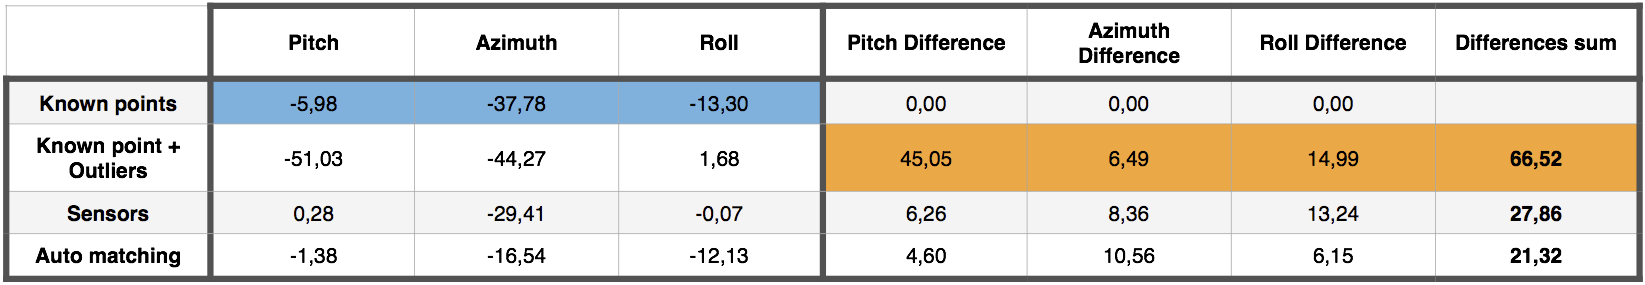
\includegraphics[width=0.95\textwidth]{rot_tests_02}
    \caption[Rotation tests comparison in Sensor only based approach -2nd example]{Rotation tests comparison in Sensor only based approach for 0.jpg and 2.jpg images. In first raw reference angles were calculated for proper point matching. Next raw shows how outliers influence those measurements. 3rd shows calculation using Sensor Fusion approach and 4th one measurements from automatic OpenCV supported matching. All angle differences are referenced to 1st row.}
    \label{fig:rot_tests_02}
\end{figure}
\subsection{Translation calculation tests}
Implemented heuristic for movement tend to be more predictable than solely relaying on Sensor Fusion Linear Acceleration usage as described in \cite{indoorPosition}. Tests for this heuristic were conducted on 4 different walking distances on flat earth surface: 1m, 2m, 5m and 10m. In figure \ref{fig:distance_tests} results are presented.
\begin{figure}[h!]
    \centering
    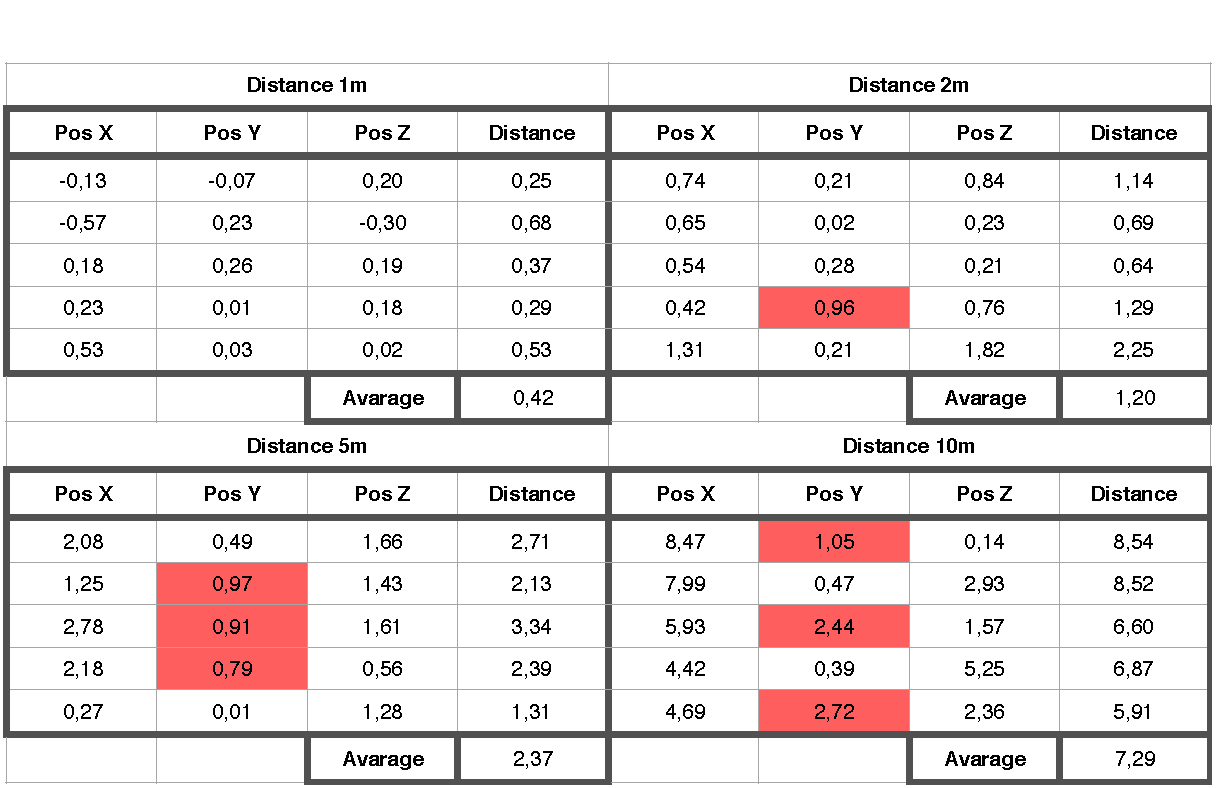
\includegraphics[width=0.8\textwidth]{distance_tests}
    \caption{Screenshot from table of results conducted on Sensor Fusion data based translation estimation during walking with smartphone. In red are indicated values, which were highly unexpected, especially in Y axis, which is perpendicular to earth surface}
    \label{fig:distance_tests}
\end{figure}
In all cases the distance estimated was very different than real one. For small distances it seems that proposed heuristic tends to be not sensitive enough having big difference between real and estimated distance traveled. Things are getting a little bit better for longer distances giving values that are much closer to real ones. However in some cases due to unbalanced up-down movement during walking "Pos Y", which is position in an axis perpendicular to earth surface, big distances are visible (Tests were conducted on a flat surface and it shows how big double  integration of acceleration over time errors can be in reality). \\
The only thing that can be said, that in a case of unpredictable movement like walking it's hard to relay on translation estimation with usage of Sensor Fusion estimation. 
\subsection{Epipolar line calculation}
To get reader acquainted, how small errors in either rotation or translation influence calculation and visualisation of epipolar lines for all of test cases from \ref{fig:rot_tests_01} and \ref{fig:rot_tests_02} adequate calculations were made. In figures \ref{fig:f_01_epi} - \ref{fig:f_02_sensor} reader can see, how big those differences can be depending on method that was used. Methods that are image based, which means that \textbf{F} was calculated directly from points correspondeces give much accurate epipolars. In case of \ref{fig:f_01_sensor} and \ref{fig:f_02_sensor} were \textbf{F} was calculated from sensor fusion estimated \textbf{R} and \textbf{T} completely miss automatically matched point correspondeces. Evaluation of time efficiency and numerical accuracy are conducted in Chapter \ref{sec:Testin2Views}. \\
At this point of his research, author had an idea to try slightly different approach, which could produce quite good effects - usage of Sensor Fusioned rotation estimation and calculating missing translation information from image itself. 
\begin{figure}[h!]
    \centering
    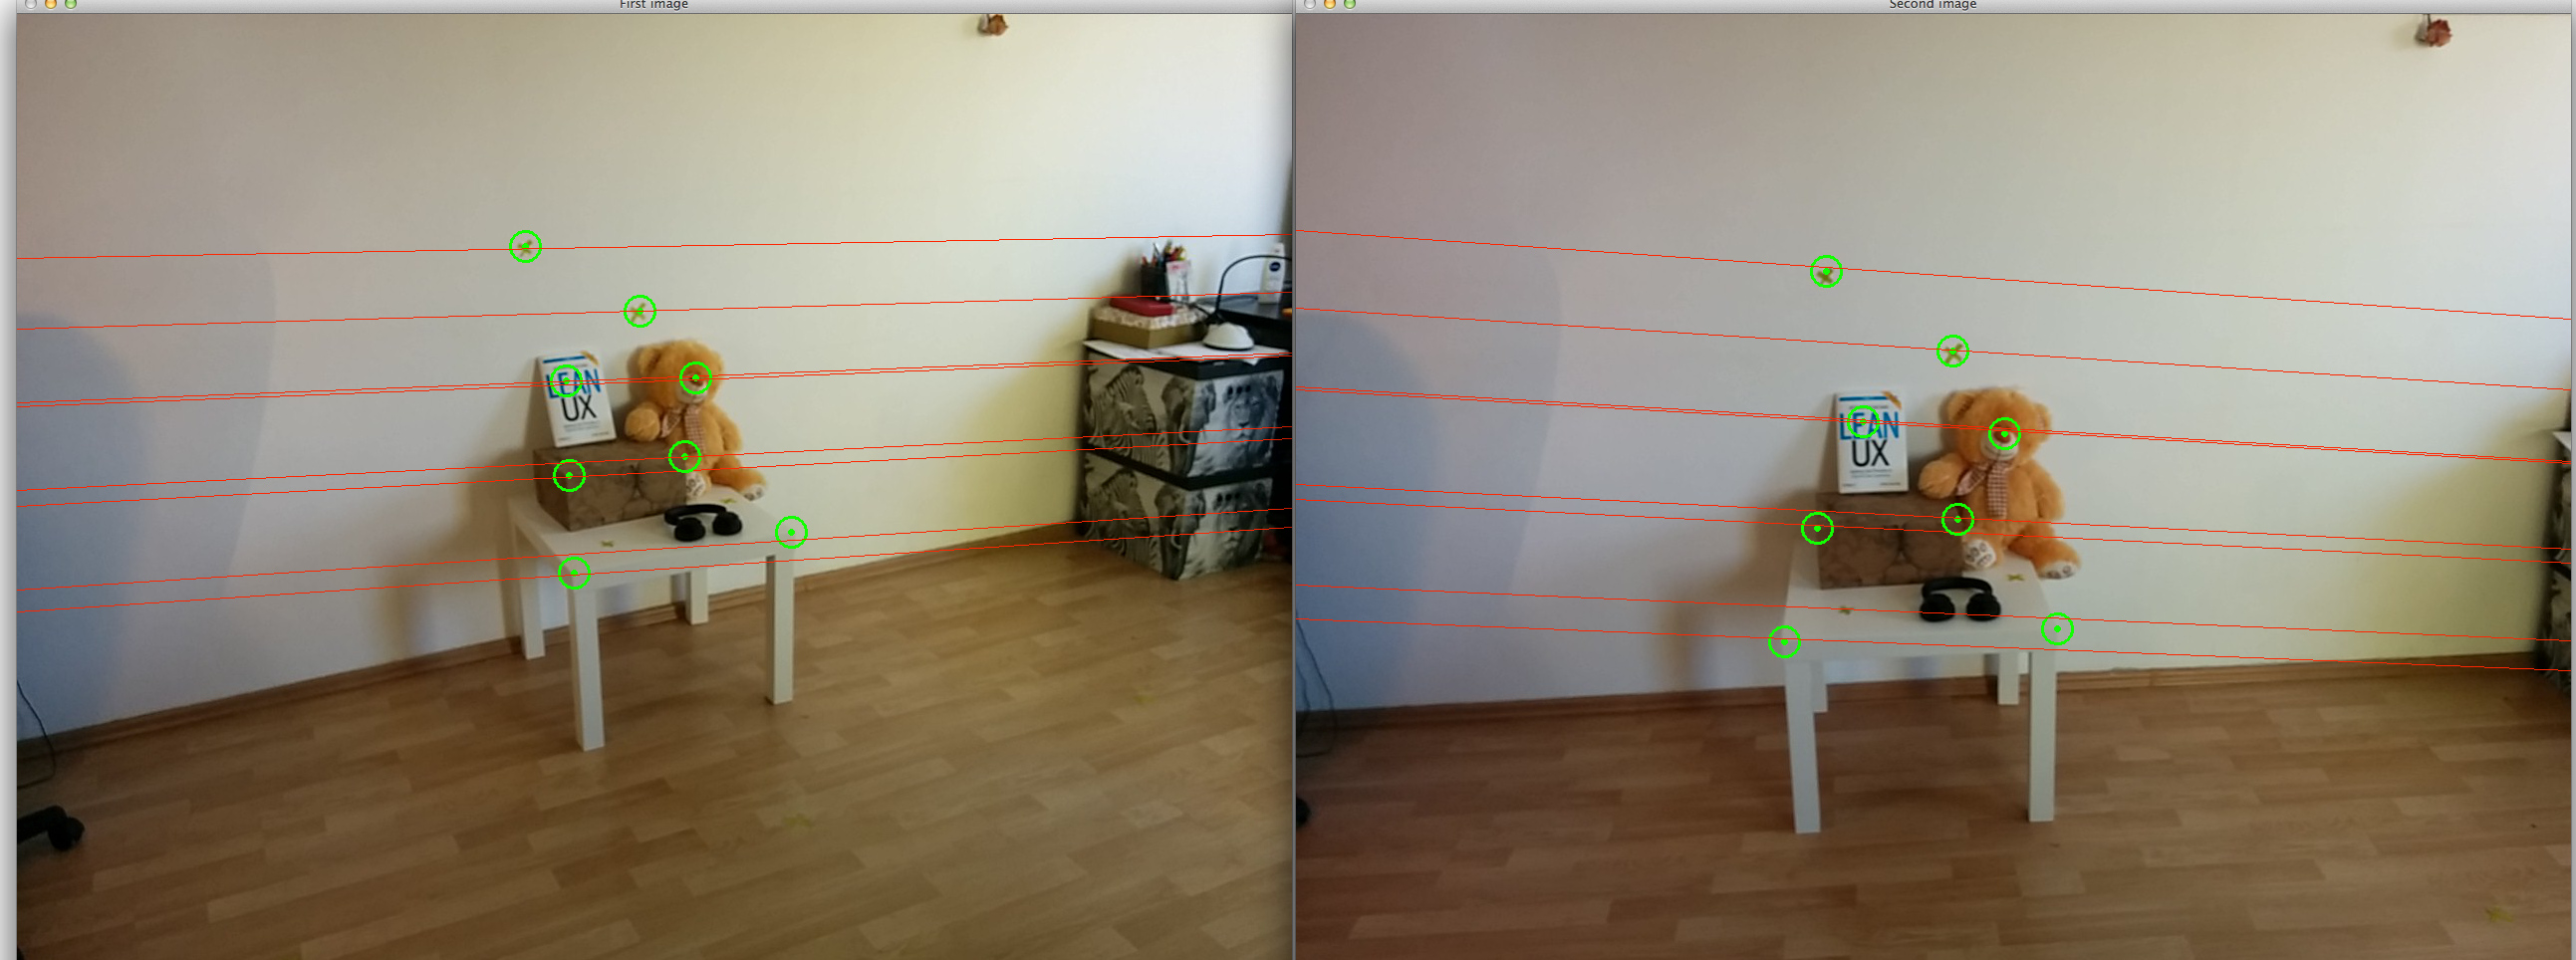
\includegraphics[width=0.8\textwidth]{f_01}
    \caption[Visualisation of epipolar lines for 8-point Fundamental matrix estimation - 1st example]{Visualisation of epipolar lines for 8-point Fundamental matrix estimation from manually selected points for images 0.jpg and 1.jpg in test dataset. No outliers are produced.}
    \label{fig:f_01_epi}
\end{figure}

\begin{figure}[h!]
    \centering
    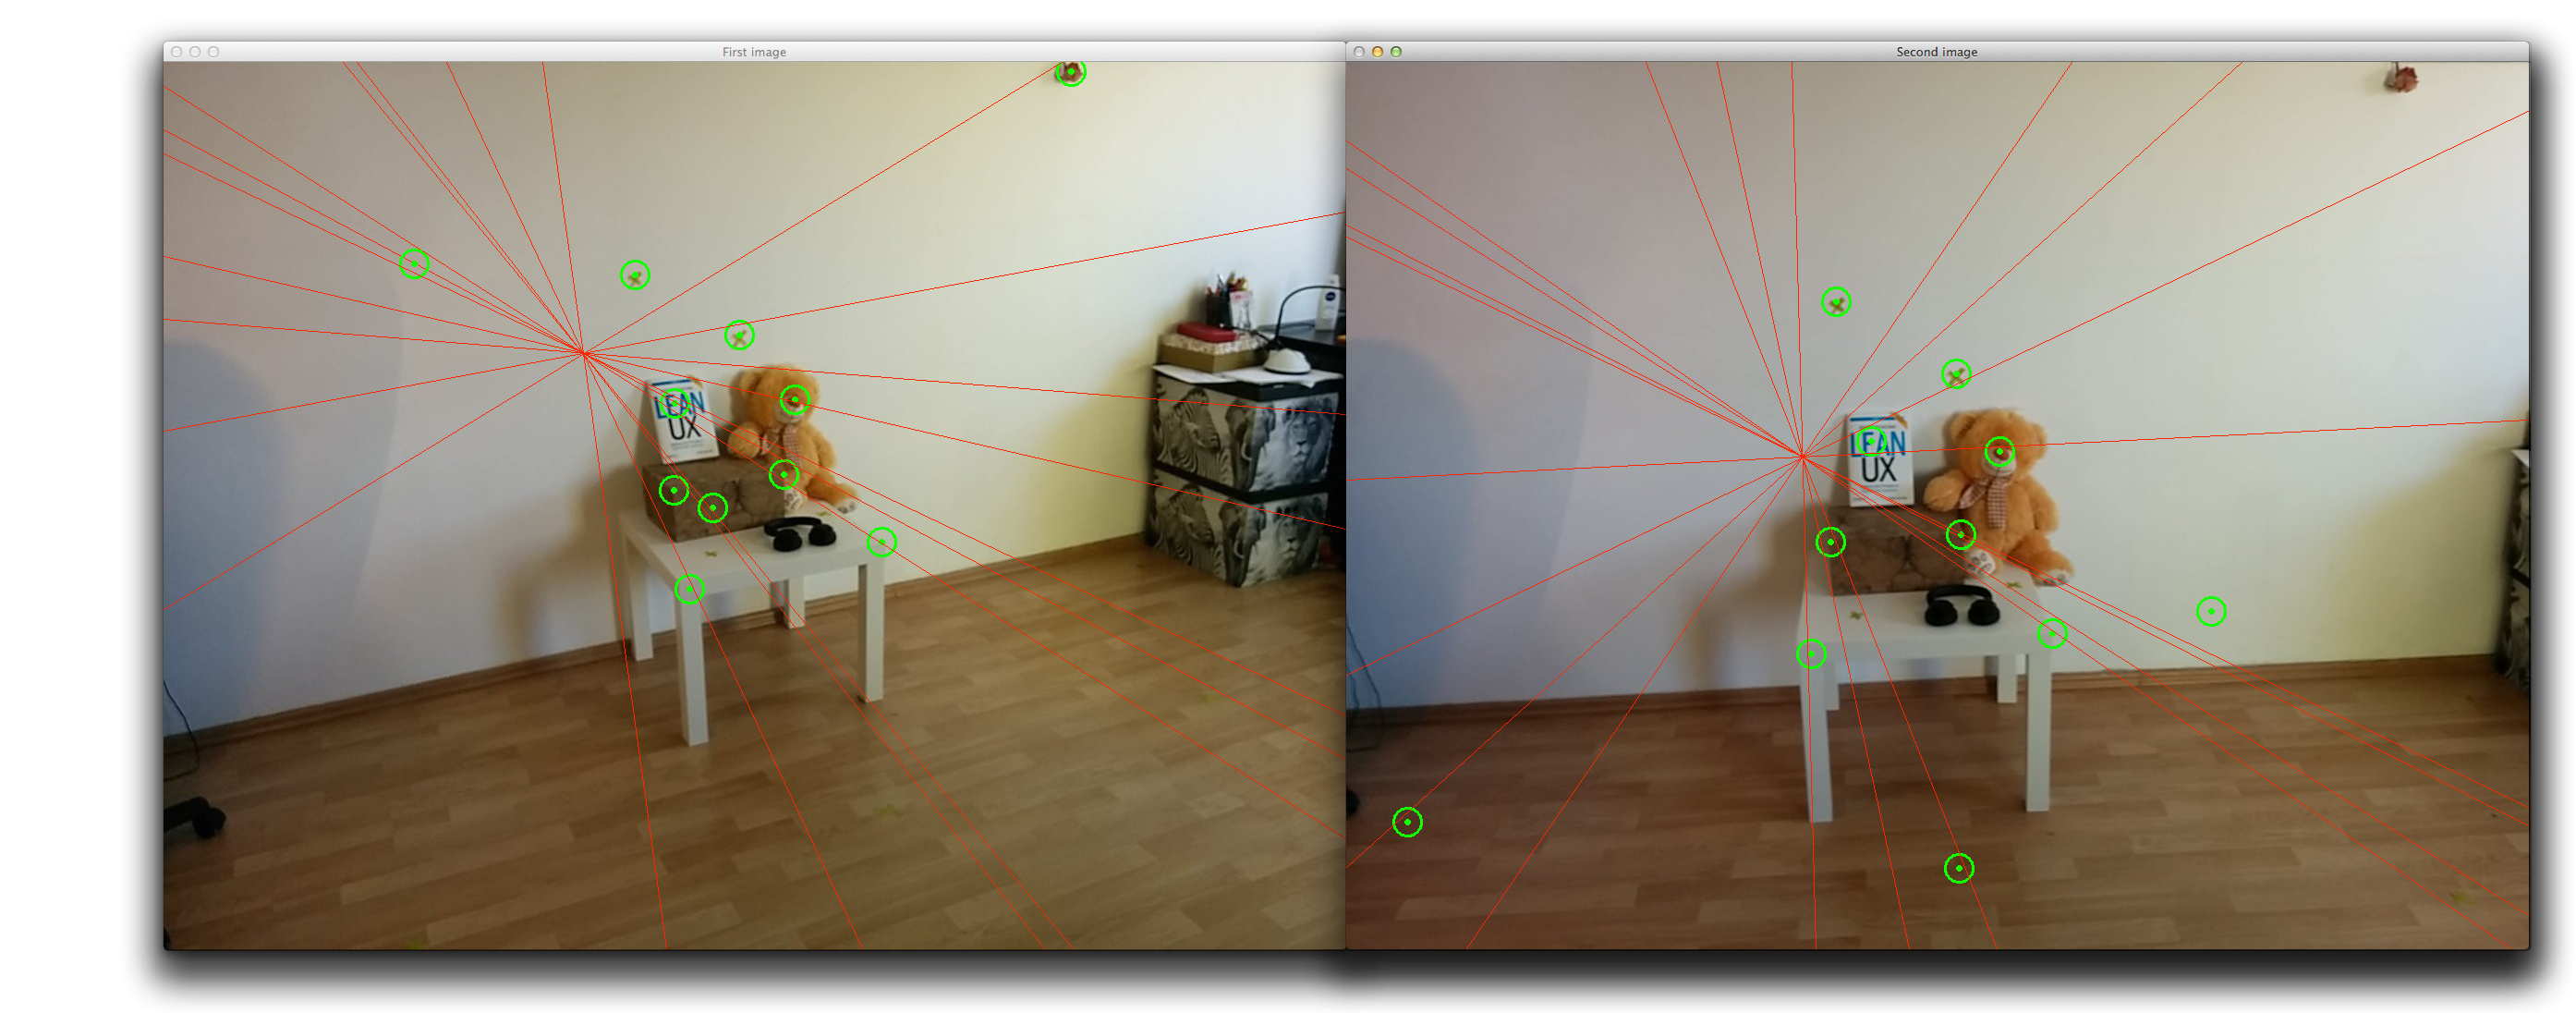
\includegraphics[width=0.8\textwidth]{01_matching_outliers_epi}
    \caption[Visualisation of epipolar lines for 8-point Fundamental matrix estimation with outliers - 1st example]{Visualisation of epipolar lines for 8-point Fundamental matrix estimation from manually selected points for images 0.jpg and 1.jpg in test dataset. Some outliers are produced and indicated by yellow lines.}
    \label{fig:01_matching_outliers_epi}
\end{figure}

\begin{figure}[h!]
    \centering
    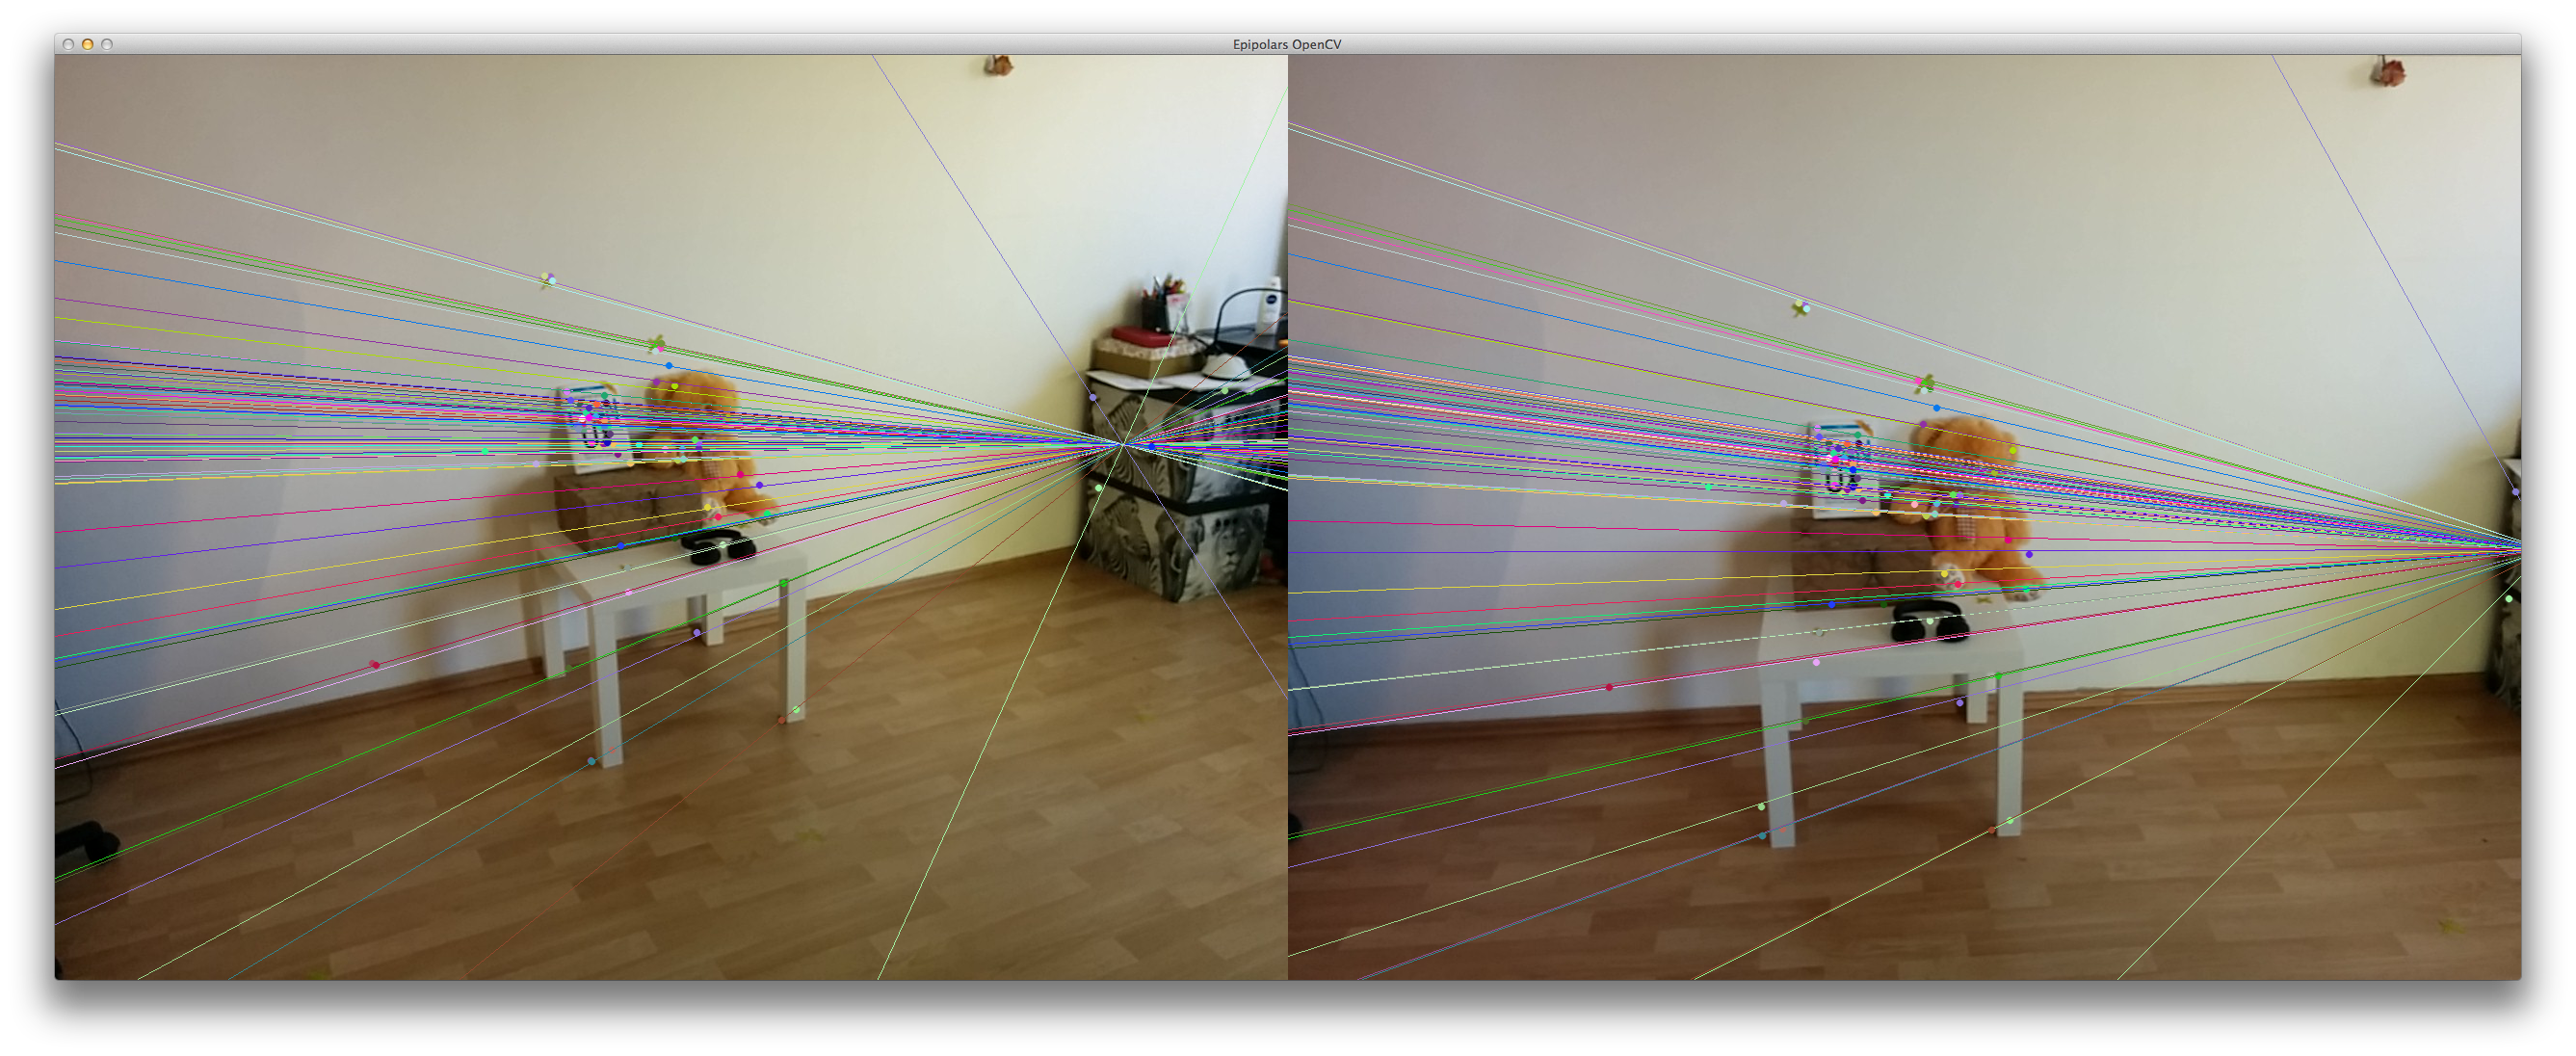
\includegraphics[width=0.8\textwidth]{f_01_8point}
    \caption[Visualisation of epipolar lines for 8-point Fundamental matrix estimation with outliers from automiatically matched correspondences - 1st example]{Visualisation of epipolar lines for 8-point Fundamental matrix estimation from automatically matched points for images 0.jpg and 1.jpg in test dataset. Some outliers are produced during feature matching process.}
    \label{fig:f_01_8point}
\end{figure}

\begin{figure}[h!]
    \centering
    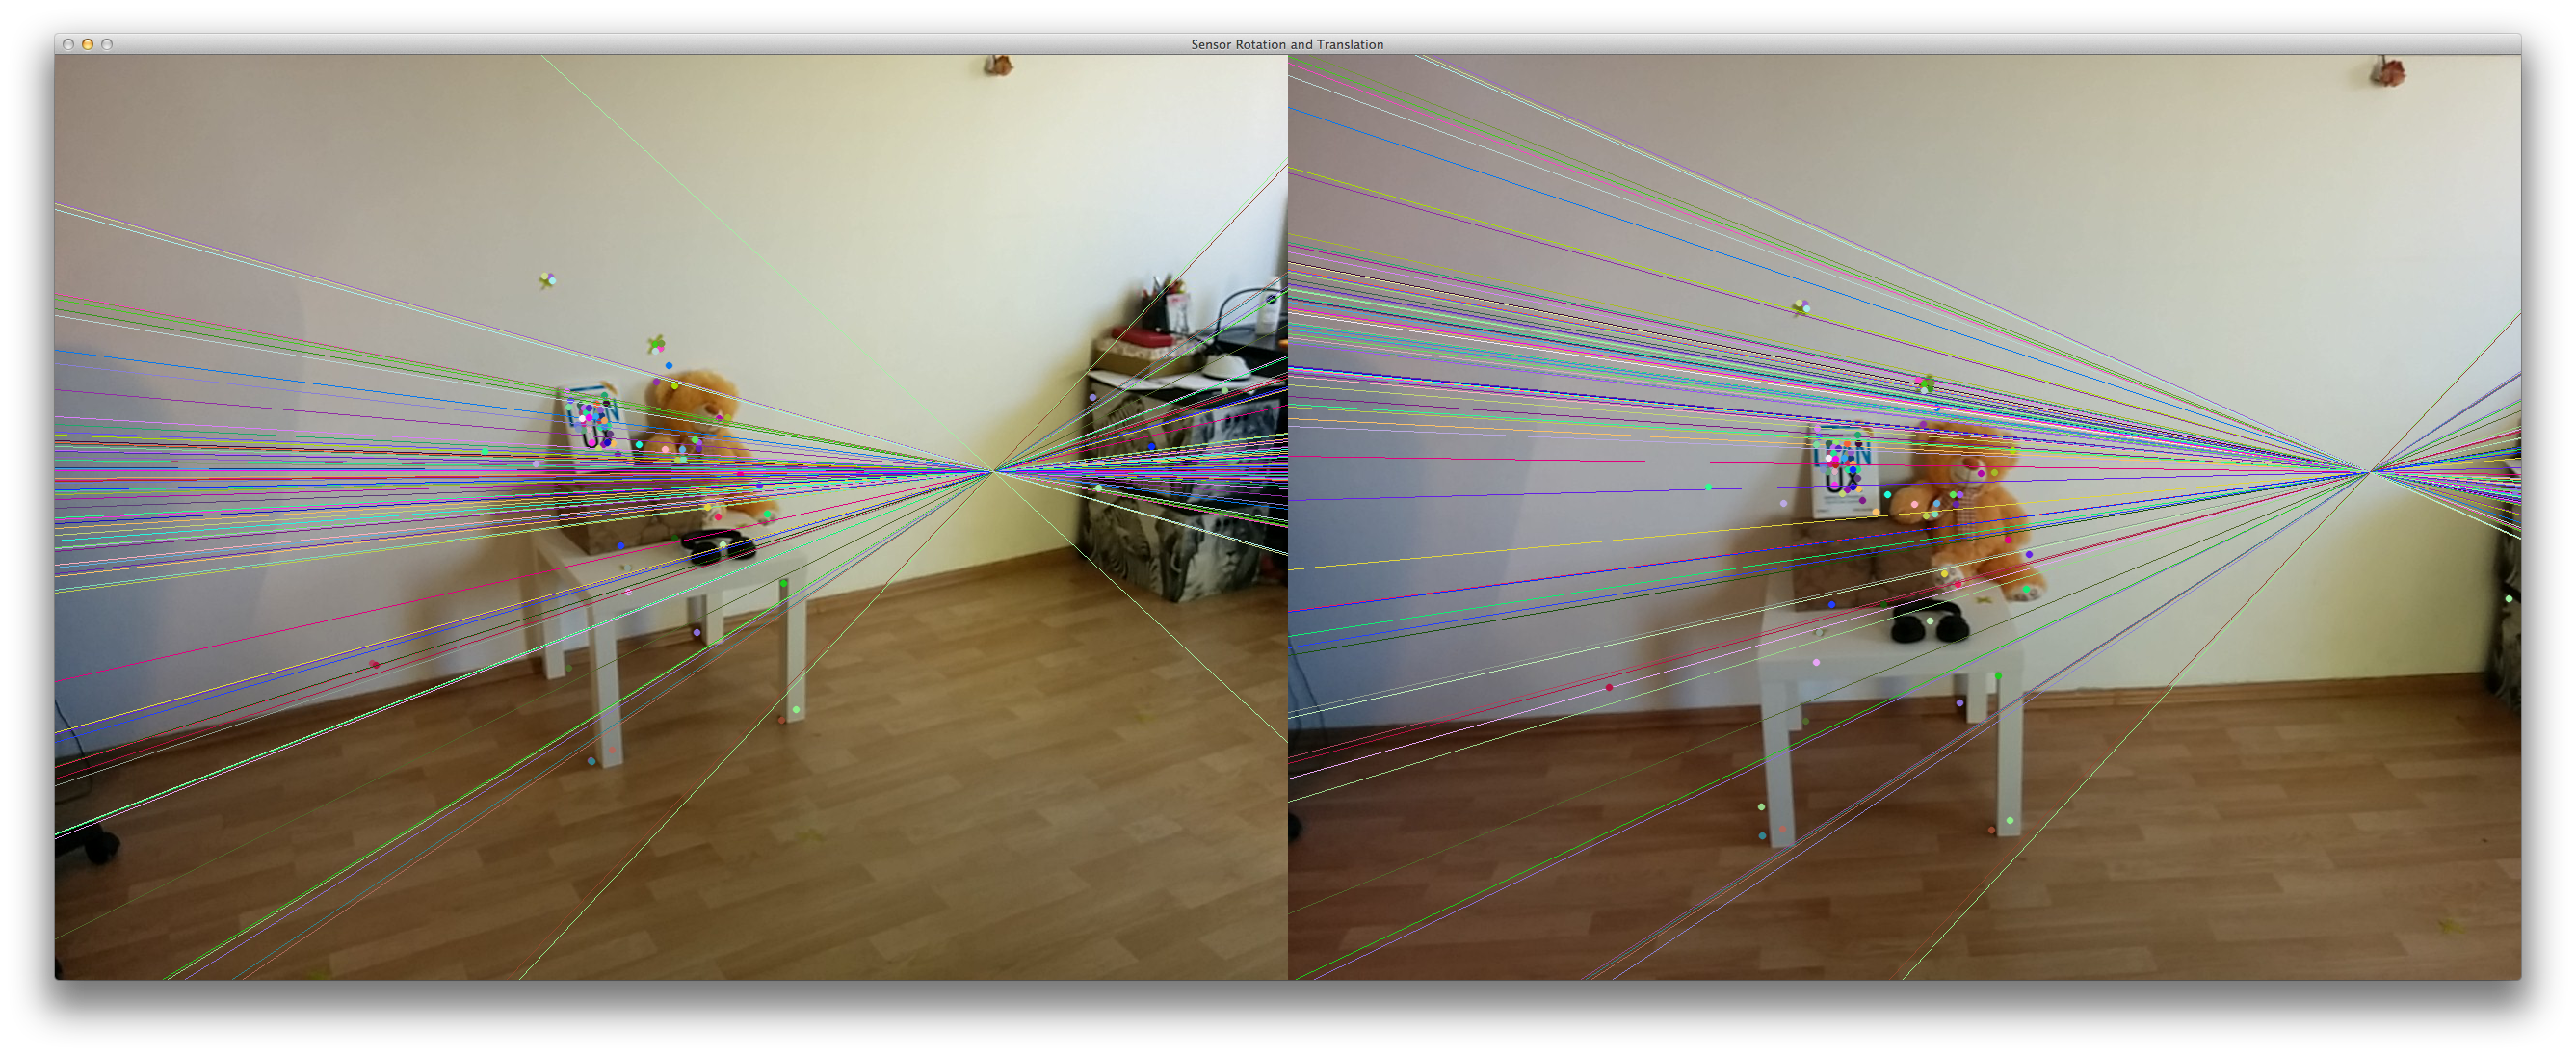
\includegraphics[width=0.8\textwidth]{f_01_sensor}
    \caption[Visualisation of epipolar lines calculated from rotation and translation estimated from Sensor Fusion readings - 1st example]{Visualisation of epipolar lines calculated from rotation and translation estimated from Sensor Fusion readings and automatically matched correspondeces for images 0.jpg and 1.jpg from test dataset. Some outliers are produced during feature matching process, but they do not disturb calculation for proper matches.}
    \label{fig:f_01_sensor}
\end{figure}

\begin{figure}[h!]
    \centering
    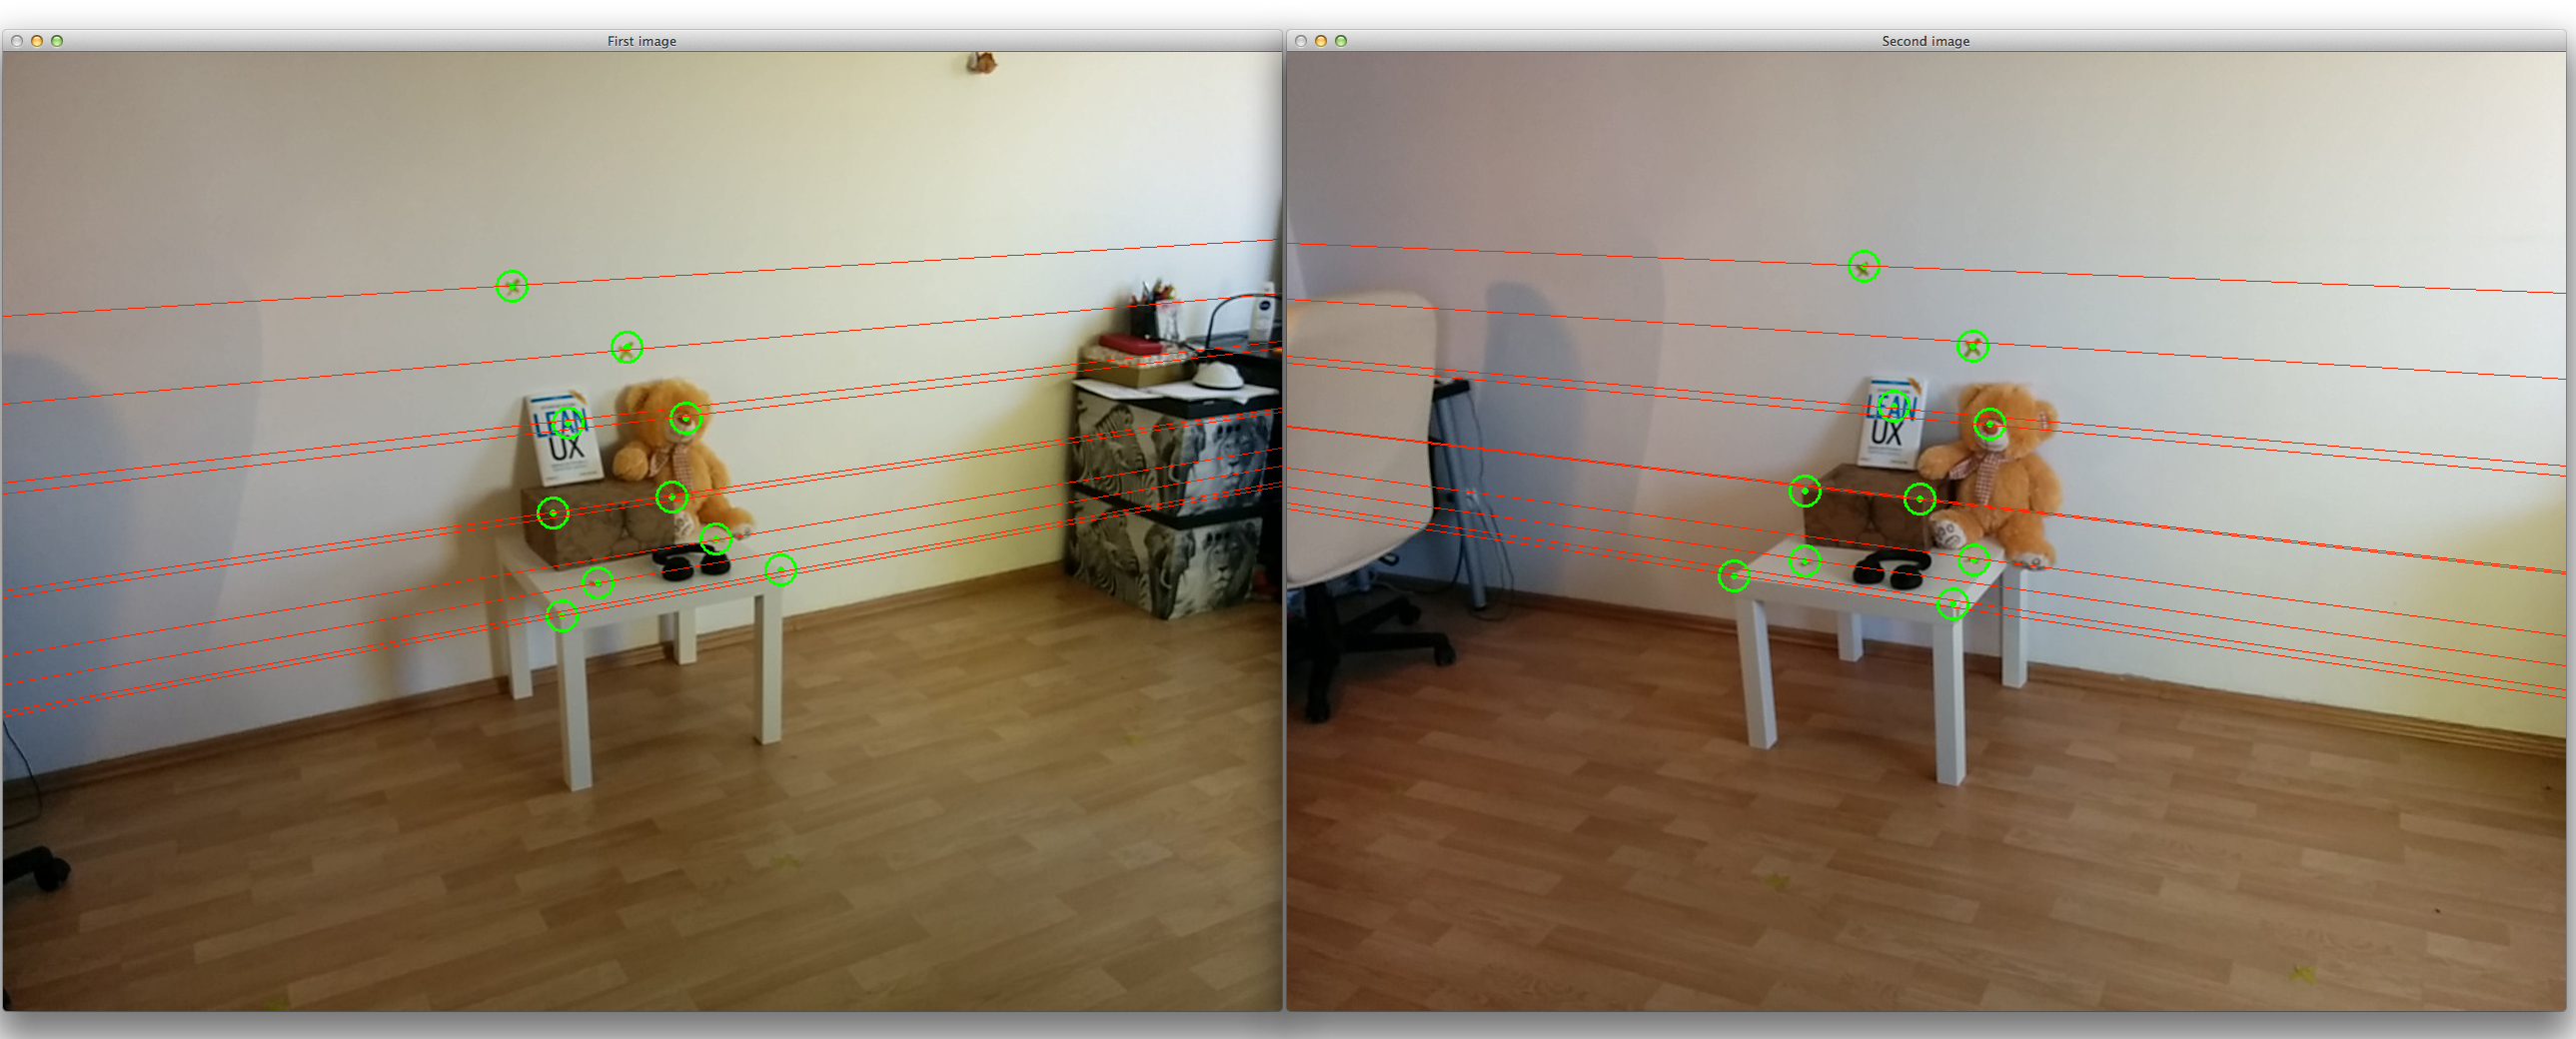
\includegraphics[width=0.8\textwidth]{f_02}
    \caption[Visualisation of epipolar lines for 8-point Fundamental matrix estimation - 1st example]{Visualisation of epipolar lines for 8-point Fundamental matrix estimation from manually selected points for images 0.jpg and 2.jpg in test dataset. No outliers are produced.}
    \label{fig:f_02_epi}
\end{figure}

\begin{figure}[h!]
    \centering
    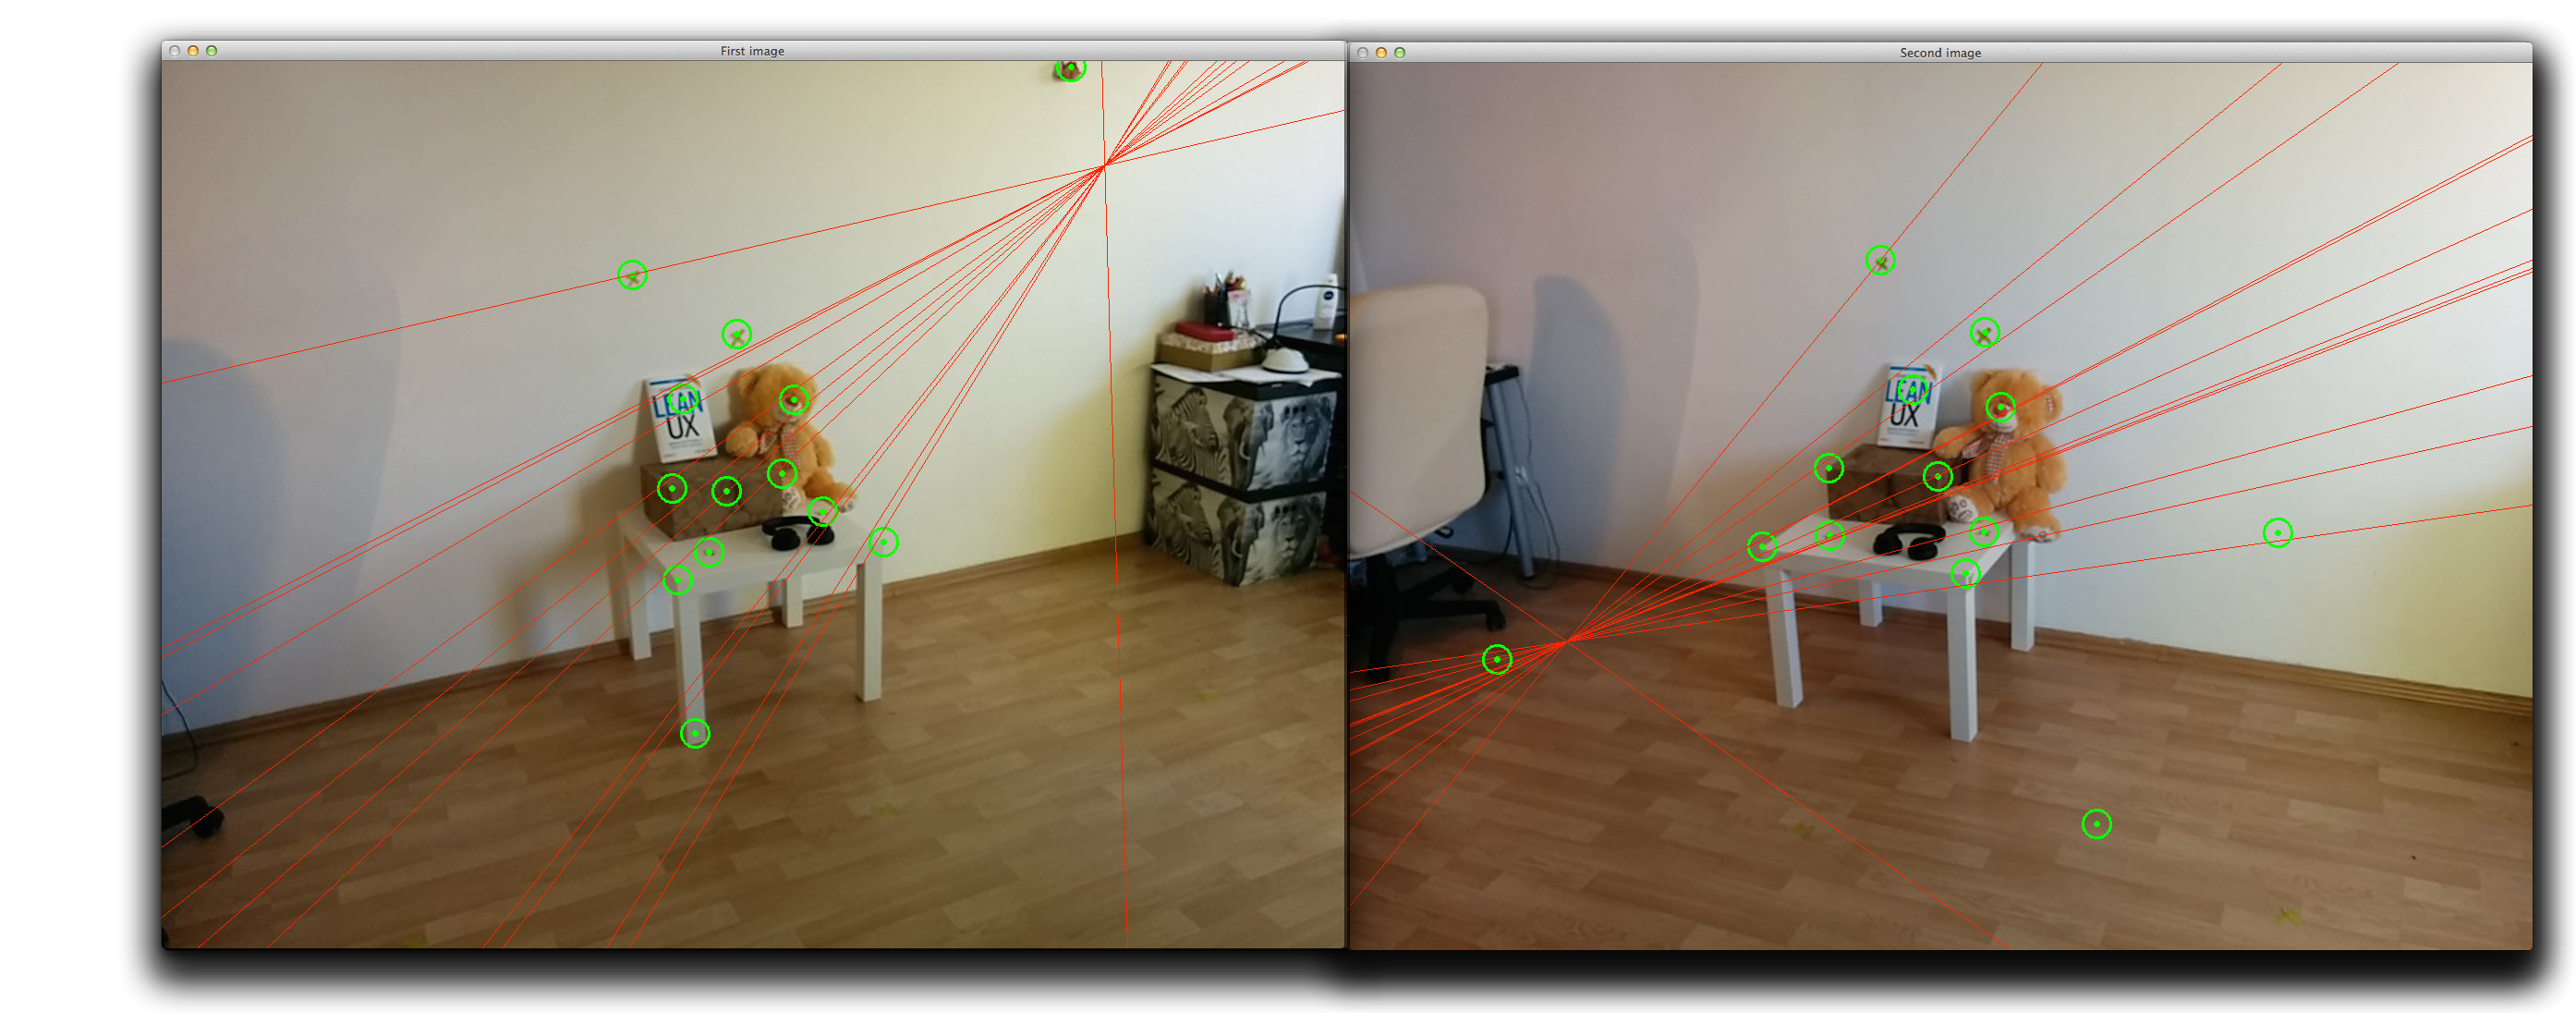
\includegraphics[width=0.8\textwidth]{02_matching_outliers_epi}
    \caption[Visualisation of epipolar lines for 8-point Fundamental matrix estimation with outliers - 1st example]{Visualisation of epipolar lines for 8-point Fundamental matrix estimation from manually selected points for images 0.jpg and 2.jpg in test dataset. Some outliers are produced and indicated by yellow lines.}
    \label{fig:02_matching_outliers_epi}
\end{figure}

\begin{figure}[h!]
    \centering
    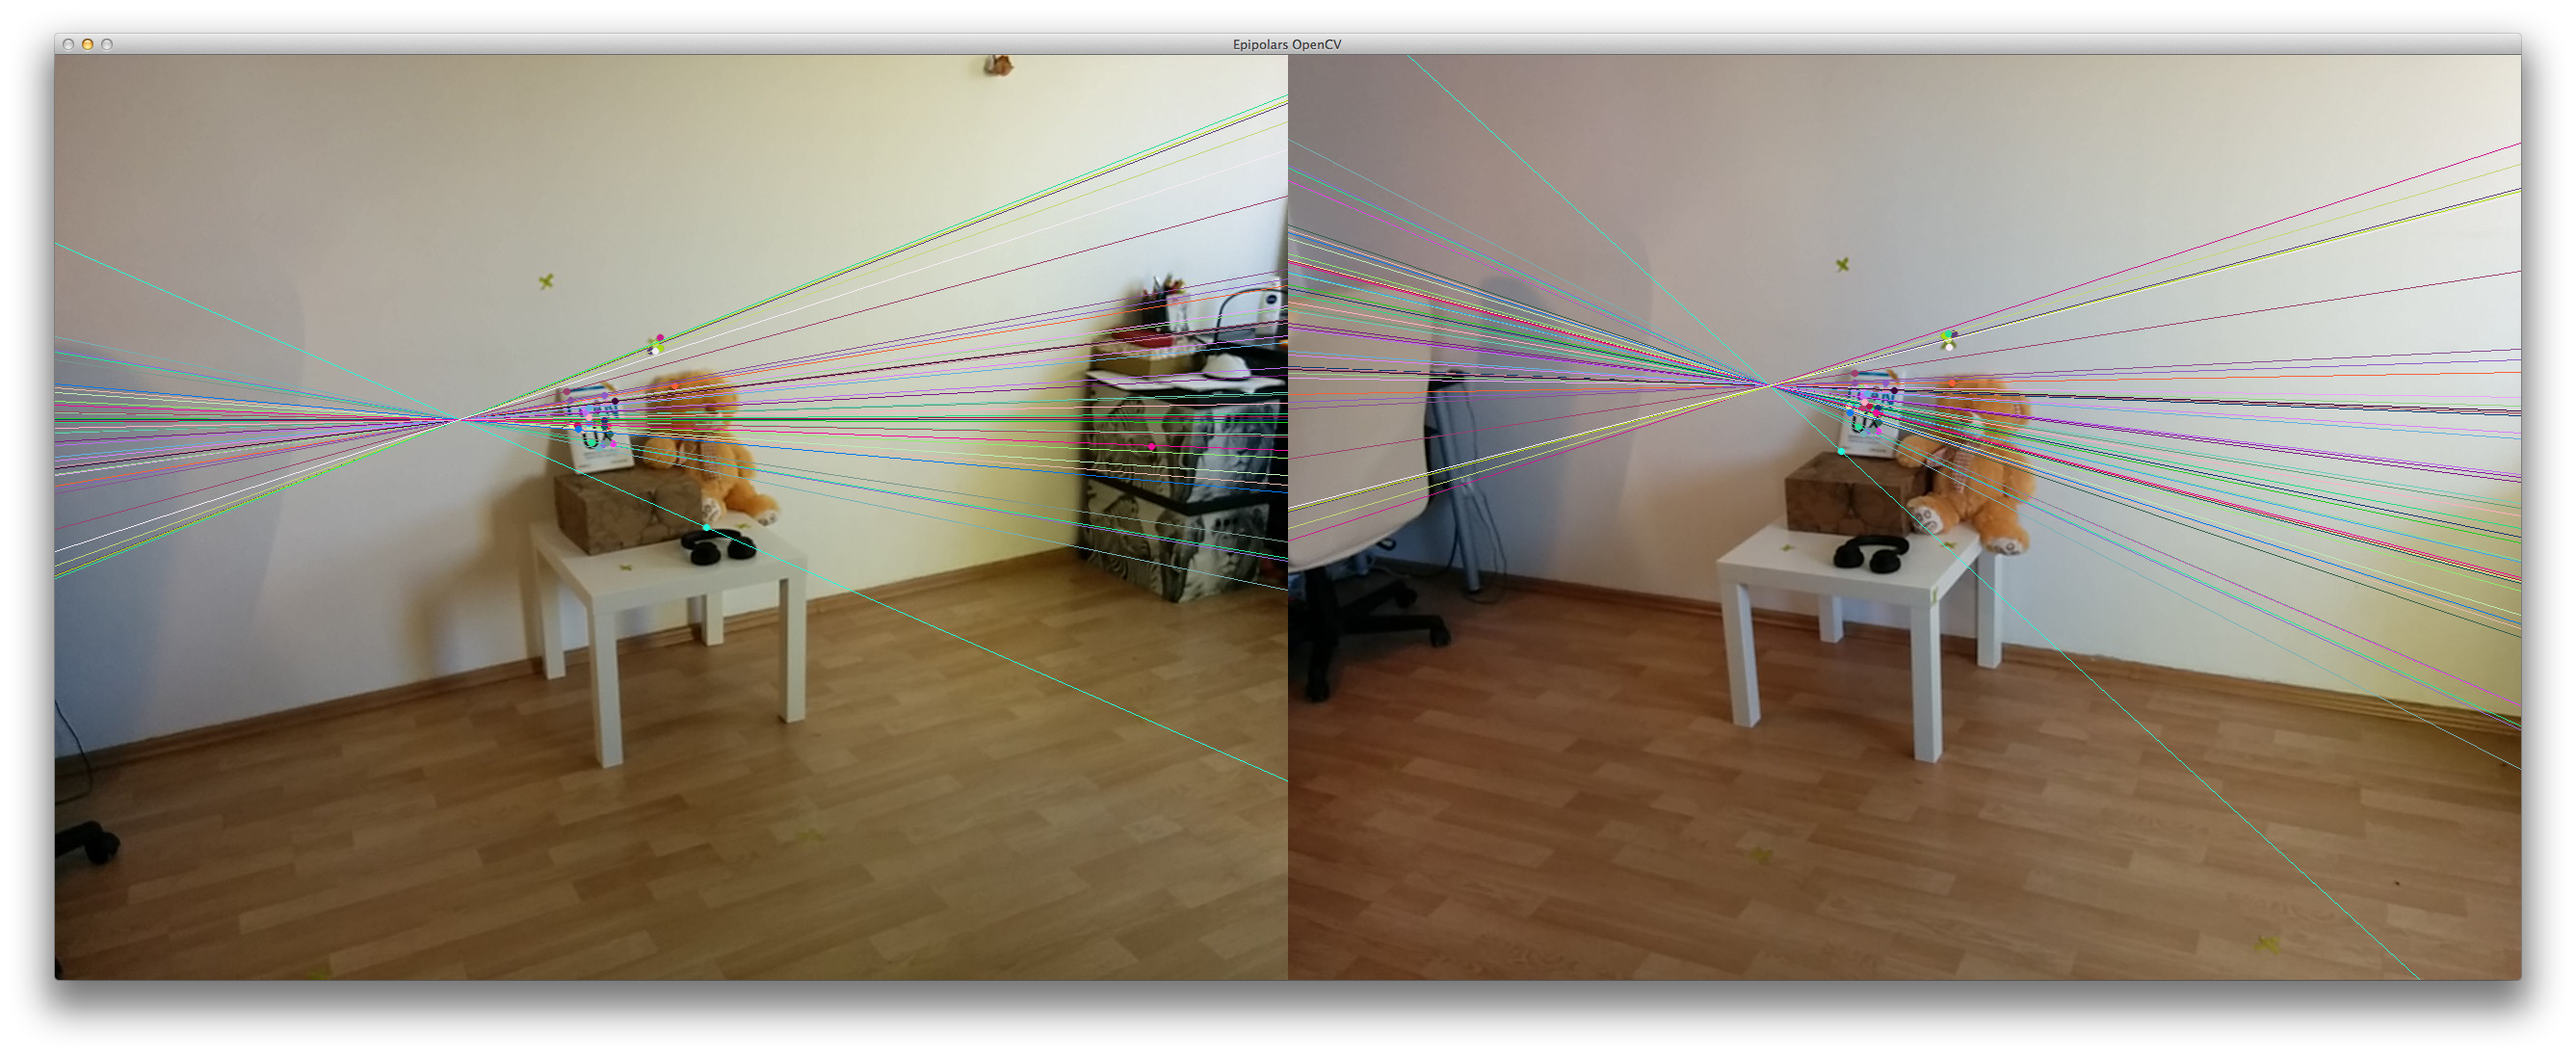
\includegraphics[width=0.8\textwidth]{f_02_8point}
    \caption[Visualisation of epipolar lines for 8-point Fundamental matrix estimation with outliers from automiatically matched correspondences - 1st example]{Visualisation of epipolar lines for 8-point Fundamental matrix estimation from automatically matched points for images 0.jpg and 2.jpg in test dataset. Some outliers are produced during feature matching process.}
    \label{fig:f_02_8-point}
\end{figure}

\begin{figure}[h!]
    \centering
    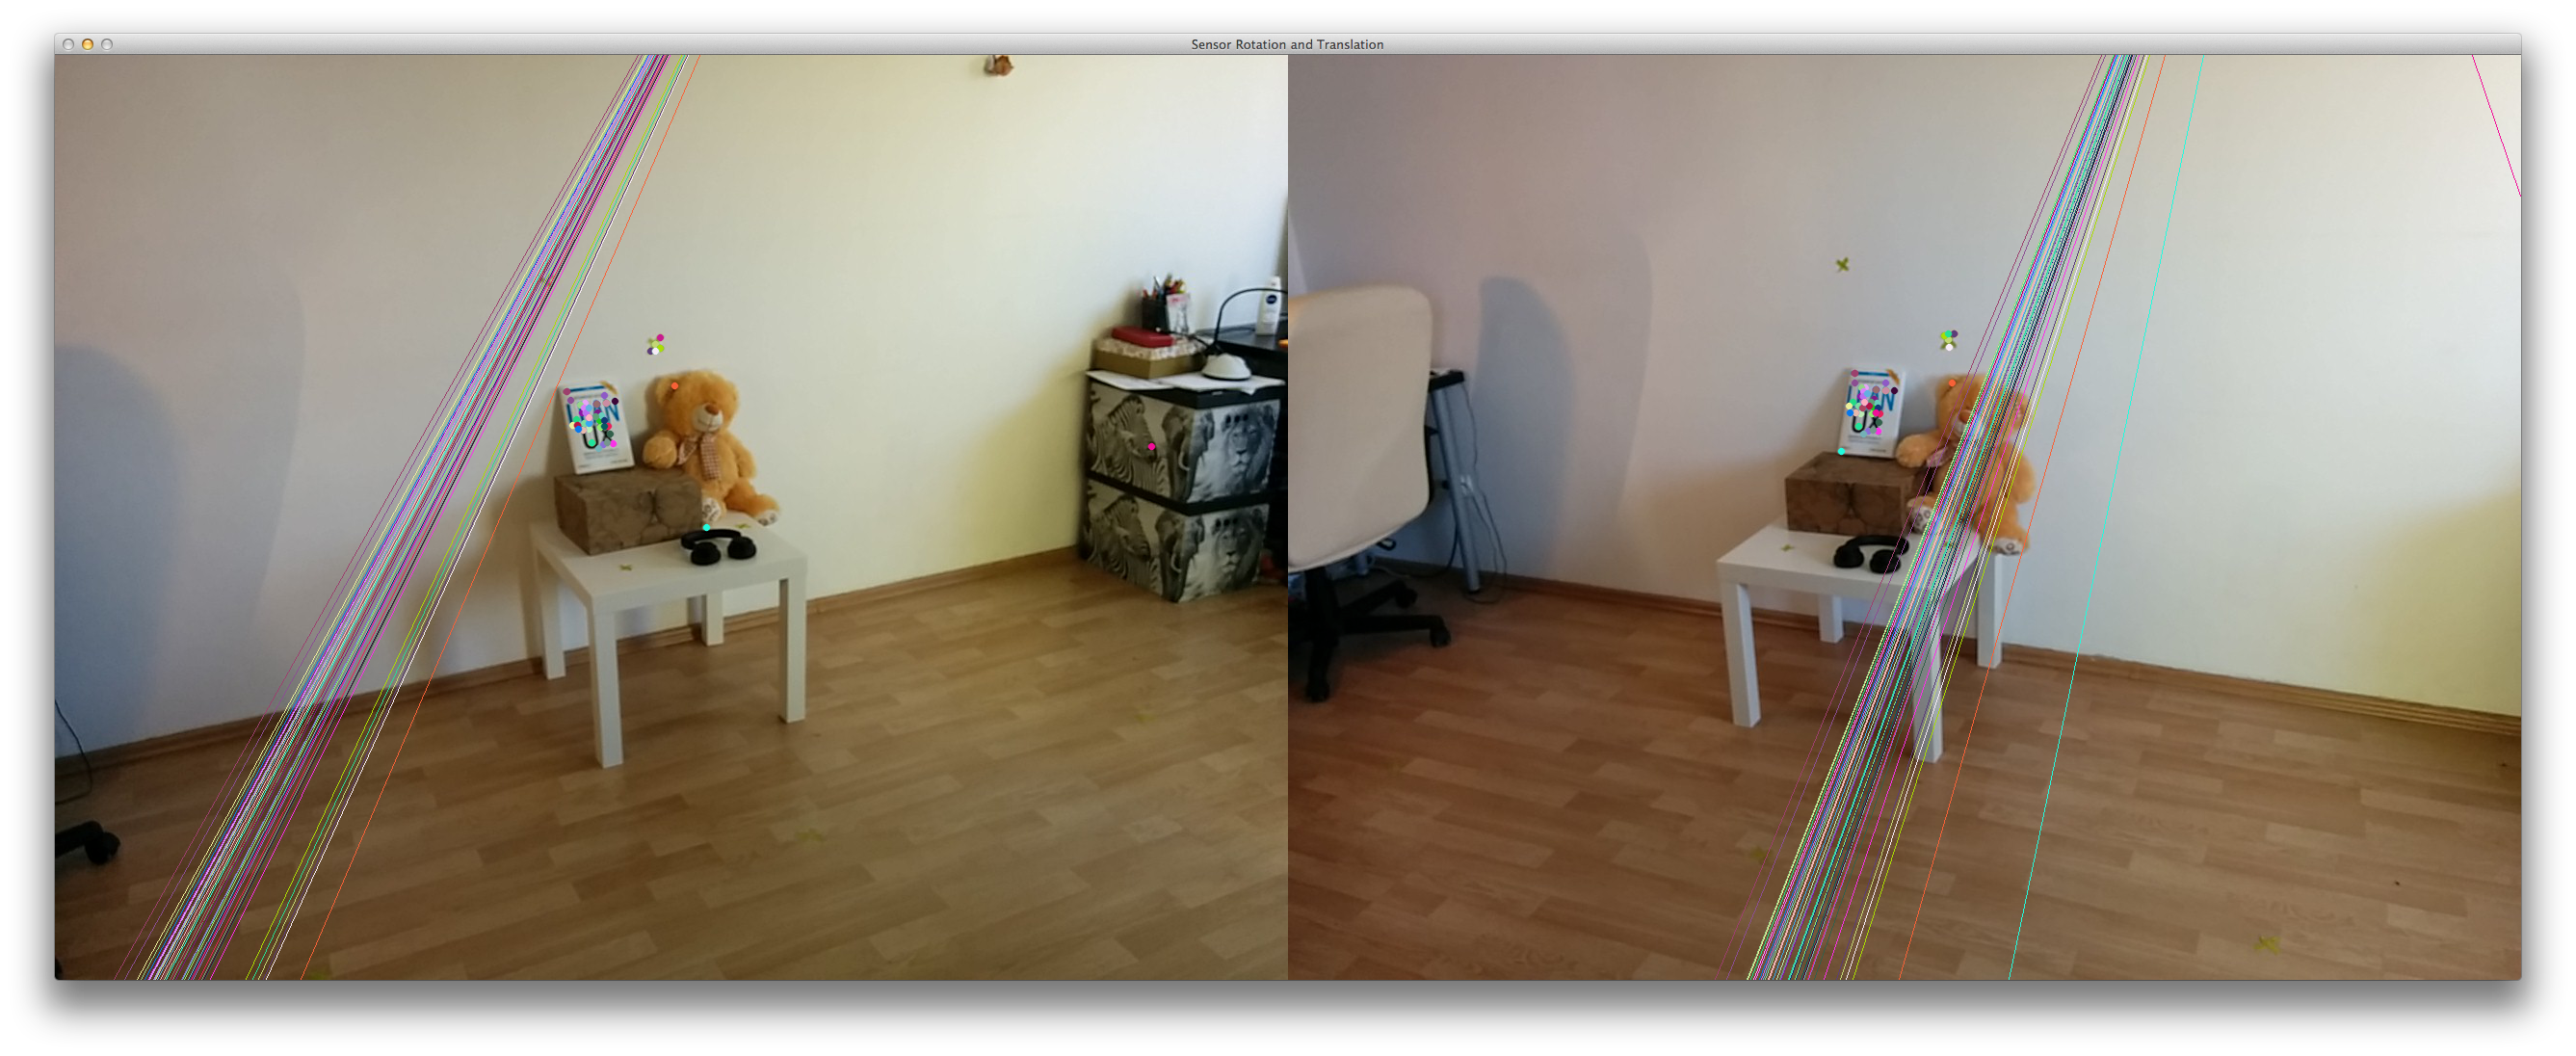
\includegraphics[width=0.8\textwidth]{f_02_sensor}
    \caption[Visualisation of epipolar lines calculated from rotation and translation estimated from Sensor Fusion readings - 2nd example]{Visualisation of epipolar lines calculated from rotation and translation estimated from Sensor Fusion readings and automatically matched correspondeces for images 0.jpg and 2.jpg from test dataset. Some outliers are produced during feature matching process, but they do not disturb calculation for proper matches.}
    \label{fig:f_02_sensor}
\end{figure}
\clearpage
% ---------------------------------------------------------------------------
%: ----------------------- end of thesis sub-document ------------------------
% ---------------------------------------------------------------------------

